\documentclass[12pt]{article}
\usepackage{preamble}

\pagestyle{fancy}
\fancyhead[LO,LE]{Физические основы компьютерных \\ и сетевых технологий}
\fancyhead[RO,RE]{Лекции Зинчика А. А.}

\fancyfoot[L]{\scriptsize исходники найдутся тут: \\ \url{https://github.com/pelmesh619/itmo_conspects} \Cat}

\renewcommand{\thesection}{}

\begin{document}

    \tableofcontents
    \clearpage

    % begin physics3_2025_09_01.tex





\section{1. Поляризация}

В прошлом семестре мы говорили о плоских бесконечных волнах. В реальности волны не бесконечные -- о них говорят, как о импульсе, одиночном, кратковременном возмущении

Свет излучается атомами за конечное время, порядка наносекунд. Получаем конечный световой импульс, длину распространения которого можно посчитать -- $l = c \cdot t$, а значит мы можем говорить о световом импульсе, который локализован, как о частице. Здесь появляется понятие кванта: атом не может излучить меньше одного фотона, поэтому фотон -- это квант, неделимая часть

Из прошлого семестра мы знаем, что электрон может преодолеть потенциальный барьер, действуя как волна, из-за своего размера. Следствием этого является ограничением на размер транзистора

Такой эффект не сходится с представлениями классической физики. В классической физике (в том числе в механике Ньютона) рассматриваются более высокие порядки размеров и на более низких скоростях, чем скорость света.
В механике Гамильтона, основывающейся на концепции гамильтониана (оператора полной энергии) отпадает понятие траектории

\mediumvspace

Будем говорить, что волна представляет $E(z, t) = \RE(E_0 e^{i(\omega t - kz)})$

Если волна не лежит в системе координат, то добавляют матрицу поворота: $E(z, t) = \RE\left(E_0 \begin{pmatrix}\cos \theta \\ \sin \theta \end{pmatrix} e^{i(\omega t - kz)}\right)$

\smallvspace

Свет считается \textbf{поляризованным}, если направления колебания светового вектора $\vec E$ упорядочены каким-либо образом

% TODO картинка

В простом случае поляризация бывает линейной (или плоской) -- в этом случае вектор напряженности движется в одной плоскости

Большинство бытовых источников света излучают неполяризованные волны -- в них колебания разных направлений быстро и беспорядочно сменяют друг друга. С помощью устройства с названием \textbf{поляризатор} можно получить поляризованный свет, поглощая другие. Поляризатор лишь частично задерживающий колебания, перпендикулярные к его плоскости, называется несовершенным. Качество поляризатора зависит от толщины и материала

С помощью другого прибора -- монохроматора -- можно получить монохроматическую волну. Так как свет с разной длиной волны имеет разные коэффициенты преломления, то монохроматор способен пропускать свет с нужной длиной волны

Если свет поляризован плохо, то его называют \textbf{частично поляризованным}

% TODO картинка

Если пропустить частично поляризованный свет через поляризатор, прибора вокруг направления луча интенсивность прошедшего света будет изменяться от $I_\min$ до $I_\max$. Причем, так как поляризатор симметричен, то угол между $I_\min$ и $I_\max$ равен $\frac{\pi}{2}$

Степенью поляризации $P = \frac{I_{\max} - I_\min}{I_{\max} + I_\min}$ можно выразить, насколько сильно поляризован свет 

\mediumvspace

Однако, так как поляризатор не пропускает лучи в неправильном направлении, то интенсивность света уменьшиться. \textbf{Закон Малюса} гласит, что доля интенсивность выходящего света от интенсивность входящего равна $\cos^2 \varphi$, где $\varphi$ -- угол между плоскостью поляризатора и плоскостью колебания $\vec E$

\[I = I_0 \cos^2 \varphi\]

Если пропустить естественный свет через поляризатор, то интенсивность выходящего света равна $I = \frac{1}{2} I_0$. Это объясняется тем, что в естественном свете волны направлены во все стороны равновероятно, а среднее значение $\cos^2 \varphi$ равна $\frac{1}{2}$

\mediumvspace

Существует круговая (или эллиптическая) поляризация, когда вектор $\vec E$ вращается в плоскости, перпендикулярной направлению распространения волны


% end physics3_2025_09_01.tex

% begin physics3_2025_09_08.tex





Всего существуют 3 способа поляризации:

\begin{enumerate}
    \item Поглощение (или дихроизм): свет проходит через вещество с длинными нитевидными молекулами. Проходя вдоль молекулы, свет свободно проходит, а поперек молекул свет не проходит

    Большинство таких линейных поляризаторов (или так называемых поляроидов) состоят из полимерной пленки или частиц кристаллов турмалина или герапатита в нитроцеллюлозной пленке

    \item Преломление: в призме Николя используется двойное лучепреломления света. В ней используется анизотропный кристалл исландского шпата, в котором

    \begin{itemize}
        \item лучи, поляризованные горизонтально, имеют показатель преломления $n_o = 1.66$ -- их называют обыкновенными
        \item лучи, поляризованные вертикально, имеют показатель преломления $n_o = 1.51$ -- их называют необыкновенными
    \end{itemize}

    Призма Николя представляет собой две одинаковые треугольные в сечении призмы. Обыкновенный луч испытывает полное внутреннее отражение от склеивающего слоя с $n = 1.55$ и поглощается, а необыкновенный свободно проходит через него и вторую призму, так как показатели преломления приблизительно равны

    % TODO картинка

    \item Отражение: Столетов предложил сделать поляризатор из стекла. При определенном угле падения $\alpha = \arctg n$ (известном как угол Брюстера) отраженный свет получается поляризованным. Для стекла этот угол равен примерно $59^{\circ}$, однако отраженный свет получается с интенсивностью 4\% от интенсивности входящего света.

    Столетов предложил использовать несколько стеклянных пластин, чтобы увеличить интенсивность -- данное устройство, состоящее из стопки стекла, получило название стопа Столетова

    Угол Брюстера применяется в изготовлении лазеров для получения поляризованных волн 

    % TODO картинка
\end{enumerate}

\section{2. Дисперсия света}

Дисперсией света называется зависимость показателя преломления от частоты волны света

Данных эффект был обнаружен Исааком Ньютоном при разложении света в спектр. Тогда Ньютон обнаружил, что для разных частот света (а следовательно для разных волн) показатель преломления разный, поэтому в стекле лучи разных частот двигаются с разной скоростью, на выходе призмы получается радужный спектр 

Благодаря дисперсии существует радуга: лучи Солнца, проходя под определенным углом (42 градуса над горизонтом) через капельки воды в воздухе, раскладываются в спектр и попадают на сетчатку глаза

\begin{wrapfigure}{R}{0pt}
    \includegraphics[width=6cm]{physics3/images/physics3_germanium_refractive_index}
\end{wrapfigure}

На сайте \url{https://refractiveindex.info} можно узнать показатель преломления. Например, металл германий, использующийся в тепловизорах, имеет показатель преломления 3.5-4 в инфракрасном спектре волн, что улучшает разрешение тепловизора при ограниченном объёме устройства

Подобные призмы используются в спектрометрах - приборах, позволяющих разложить свет в спектр и узнать, какие длины волн пресутсвуют в спектре

Разные газы в газоразрядной лампе излучают свет разного цвета (то есть спектр из разных длин волн). Поэтому с помощью спектрометра можно обнаружить, из чего состоит источник света (например, Солнца): зная спектр горения водорода и гелия, можно предположить концентрацию горящего вещества на поверхности Солнца

Более продвинутый прибор -- масс-спектрометр -- используется для изучения состава вещества: вещество нагревают, излученный свет попадает на масс-спектрометр, который определяет интенсивность для разных волн света

% NO ANTI-MASS SPECTROMETER? 😿 
% @@@%%%%%%%%%%%%%%@%@@@@@@@@%%%%%%%%%#%##%%@@@@%%%%%%@@@@@@@%#***#####%%%@@%@@@@@@@@@@@@@%%@@@@@@%@@@
% %%%%%@%%%%%%%%%%%%%%@%@%@@@@%%%%%#%####%@@@@@@@@%%@%@@@@@@@@@@@@%%%%%%%%@@@@@@@@@@@@%%%@@@@%@@@@@@%%
% @%%%%%@%@@%%%%%%%%%%%%%@@@@@%@%%%%%%%##%@%@@@@@@%%@@@@@@@@@@@@@@@%%%%%%%@@@@@@@@@%%%@@@%%%%@@@%@@%@%
% @%%%%%%%%%%%@@%%%%%%%%%%%%%%@%@@%%%%%%@%@%%@@@@%#%@@@@@@@@@@@@@@%###%%@@@@@@@%%%%@@%%%%@@@@@%%%@@%%@
% %%%%%%@@%@%%%%%%%@@%%%%%%%%%%%%@@@@%%%@%@%@@@@@%%%@@@@@@@@@@@@@@@@@@@@%%%%%%%%@%@%@@@@@%%%%@%@%@%%%%
% %%%%%%%@@%%%%%%%%%%%%%@%%%%%%%%%%%%%%@%@@@@@@@@%%%@@@@@@@@@@@@@@@@@@%%%@%@%@@%%@@@%%@%%%%@@%%%%@%%%%
% %%%%%%%%%%@%@%%%%%%%%%%%%%@%%%%%%%%%%@%@%@@@@@@%%%@@@@@@@@@@@@@@@@@@@%%%%%@%@@%%%@%@@%%%%%%%%%%%%%%%
% %@%%%%%%%%%%%%%%%%%%%%%%%%%%%%%@%%%%%@@%@@@@@@@%%%@@@@@@@@@@@@@@@@@@@@@@%%%%@%%%%@%%%%%%%%%%%%%%%@@@
% %%%%%%%%@@@@%%%%%%%%%%%%%%%%%%%%%%%%%@%@%@@@@@@%#%@@@@@@@@@@@@@@@@@@%%@%%%%%%%%%%%%%%%%%%%%%%%@%%%%%
% %%%%%%%%%%%%%%%@@@%%%%%%%%%%%%%%%%%%%@@%@@@@@@@%%%@@@@@@@@@@@@@@@@@@%%%%%%%%%%%%%%%%@@@%%%%%%%%%%%%%
% %%%%%%%%%%%%%%%%%%%%%%%%%%%%%%%%%%%%%@%@%@@@@@@%%%@@@@@@@@@@@@@@@@@@%%%%%%%%%%@@@%%%%%%%%%%%%%%%%%%%
% %%%%%%%%%%%%%%%%%%%%%%%%%%%%%%%%%%%%%@%@%%%%@@@%%%@@@@%%%%%%%%%@@@@%%%@%%@%%%%%%%%%%%%%%%%%%%%%%%%%%
% %%%%%%%%%%%%%%%%%%%%%%%%%%%%%%%%%%%%%@%%%%%%%@@@%#%%@%%%%%%%%%@@@@@%%%%%%%%%%%%%%%%%%%%%%%%%%%%%%%%%
% %%%%%%%%%%%%%%%%%%%%%#%%%%%%%%%%%%%%%%%@%%%%%%%@@%%%%%#####%%@@@%%%%%%%%%%%%%%%%%%%%%%%%%%%%%%%%%%%%
% @@@@%%%%%%%%##%%%%%%%%%%%%%%%%%%%%%%%%%%%%%%%%%%@%%%@%####%@@@%%%%%%%%%%%%%%%%%%%%%%%%%%%%%%%%%%%%%%
% %%%%%%%%%%%%%%%%%%%%%%%%%%%%%%%%%%%%%%%%%%%%%%%%%%#*####%@@%%%%%%%%%%%%%%%%%%%%%##%%%%%%%%%%%%%%%%%%
% %%%%%%%%%%%%%%#####%#*#####%%%%%%%%%%%%%%**#%%%%%%%@@%%%%%####*##%###%%%%%%%%##########%%###%%#%%%%%
% ###%%%%%%%%%#########**#%####%%%%%%%%%#%%***%%%%%%%%%%%@%%####**###*#%#%%%%%%###*######%%###%##%%%%%
% ####%%%%%%%%#########*#*########%%%######===******#%%%*#***##*+*###*#%####%#####*######%%###%#######
% #####%%%%##################%%#####%%#####**+**##%%*==#%%%###***#######%%%%#%%%######################
% #%%%#%%%%####*#%%%##*####*#%%#*##%%%%#*##%%#=*#%%%%=-%%%#*++*%%%######%%%%#%%#*#**#%%#*#*##**#%%%###
% ##%%####%######%%%##***####%%####%%%#######*=*#%%%#=-#%%#***##%#######%%%%#%%%#%%%%%###%####*#%%%###
% #*#%%######%%##%%%##**################*#####*+*####-=*%%%**#%%%#######%%%##%####**#%%%%%%#%%#%%%%%%#
% #%%%%###%%#%%%%#####*****##***#*######***##%#*+*#%*==##%%**###%%%######%#######***#######****#%%####
% ##%%%#######%%######**##**##%%#**##%#**%#*****++*#*==#****+*####%%#*##%%%%%###******##******######%%
% #%%%%####%######*#####*****###***#*#***##*****=*##*==#+***++***#%##**####*#%#****###*#*****######%##
% #############%%%%%%#*******************##***##*#%#+:=*****++**#*%#****###**##*****#%##****#*****####
% #######%##**########********#*+++***************%%*::=*****#######**++++**###******#*******#%%#*####
% #*##%%##*#****####********+++******************+=**:-++***%%%%%%%*****#%%**++***************#%%####*
% #*##%#****#*##**###**+++****%%%***#%%##***++*##+=*=.-=-:-=+++**++**#%%%##%##**+==+**********#####*##
% #*######%###*##**++*****#%%%%%%#%#%####%%%*++*#*=++::=+*#*+*+++==#*#########%##*+=====********###***
% ****#**#*#*#++*******%%%#%%#**#*+#%%+++******#%##==:-:=#@*#@%*+****+#**#***###*#%#**++===+*##%#*##*#
% ***#*#%%@@%@%%%%%#********++++===*%%*===*****%%@%*=:+**#%%%*+==*#%#%#%%%%%%%%%#%%%%%*#***+++++*##***
% ****#%@%%%%%%%%%*+*#******++===++*%%%****##****%%*+:=%*#%***+*#%*#%%%%%%%%%%%%%#%######%%##****++***
% ***%@%%%%%%%%%%*=+#%%%%#***#*+++++%@%%%##%%%%%%@@@#:+****##%%%%***%%%%%*#******%%########%#%%#*****+
% ##%%%%%%%%%%#%*=+*#%%#*******++++*#@@@@%%%%%%%%@@@%*###**#%%%%%@*#%##*+*****====+++***********######
% %@%%%%%%%%%%%*=+*#%%**************#%%%%%%%%%%%%%%%%@%##**#%%%%%@@%%**++++***=====+++*************#*#
% %%%%%%%%%%%%*=+**%#***********+==**%%%%%%%##%@%%%%%%%%#%#%%%%%##%%#****+*+=+==+*%*###**************#
% %%%%%%%%%%%+=+*#%%*****++*******+**##*##*#%%%%%%%%%@@%%@%%%%%%#*=---=*##*+:===+*#*****%#%#%%%@%*****
% %%%%%%%#%%*=++*#%#*********************+++*##*=*####**%@%%%@@%******+==--=*%===#%##*#*%#%%####%%#***
% %%%%%%#%%*=++*#%#**********+*++++++++++++**#+-=*##**##%@@@@@%#*++++***++**+====*#####%%%#%%%%%%%%#**
% %%%%%%%%+=++*#%%***********+++++++++++*****=-=******##%%@@@%%%#*****#***+**+===*#%*#**#%#%%%%%%%%%#*
% %%%%#%%+=++*##%%*******+=====+++++++++**#*=-=*#**+++*##%%%%%%#******+++****+====+**%#%%%@%%#%%%%@%%#
% %%%@%%*=++**#%%%****++===========++=+*##*--=+***++++*##*##%%%******++++++**#*+====+++*%#%%%%%%%%#%%@


Дисперсия возникает как следствие уравнение Максвелла. Допустим для слабопроводящей среды $\sigma, \varepsilon, \mu = \const$ ($\sigma = \frac{1}{\rho}$ -- удельная проводимость в сименсах)

По закону индукции Фарадея $\vec\nabla \times \vec E = -\mu\mu_0 \frac{\partial \vec H}{\partial t}$

$\nabla \times (\nabla \times \vec E) = -\mu\mu_0 \frac{\partial}{\partial t} (\nabla \times \vec H)$

$\nabla \times (\nabla \times \vec E) = \nabla (\nabla \vec E)$

$\nabla^2 \times \vec E = -\mu\mu_0 \frac{\partial}{\partial t} (\nabla \times \vec H)$

По теореме о циркуляции магнитного поля $\nabla \times \vec H = \sigma \vec E + \varepsilon \varepsilon_0 \frac{\partial \vec E}{\partial t}$

Получаем $\frac{\partial^2 \vec E}{\partial t^2} + \frac{\sigma}{\varepsilon \varepsilon_0} \frac{\partial \vec E}{\partial t} = v^2 \Delta \vec E$ -- волновое уравнение, где $v^2 = \frac{1}{\varepsilon \varepsilon_0 \mu \mu_0}$

Из этого волнового уравнения для волны, направленной в сторону оси $Ox$, получаем $\frac{\partial^2 E_y}{\partial t^2} = v^2 \Delta E_y - \frac{\sigma}{\varepsilon \varepsilon_0} \frac{\partial E_y}{\partial t}$

Решение его является функция $E_y = E_0 e^{i (\omega t - k x)}$, то есть $\omega^2 = v^2 k^2 - \frac{i \omega \sigma}{\varepsilon \varepsilon_0}$, где $k = \frac{2\pi}{\lambda}$ -- волновое число

Уравнение 

\[k^2 = \frac{\omega}{v^2} - \frac{i \omega \sigma}{\varepsilon \varepsilon_0 v^2}\]

называют дисперсионным (то есть зависимость $k(\omega)$). Из него $k = \pm \frac{\omega}{v} \sqrt{1 - \frac{i \sigma}{\varepsilon \varepsilon_0 \omega}}$

Для $\frac{\omega}{\varepsilon\varepsilon_0 \omega} \ll 1$ можем аппроксимировать корень, получаем $k \approx \frac{\omega}{v} \left(1 - i \frac{\sigma}{2\varepsilon\varepsilon_0 \omega}\right) = k^\prime - i k^{\prime\prime}$

В ходе вычисления получаем комплексное $k$: вещественная часть волнового числа $k^\prime$ определяет длину волны, мнимая часть $k^{\prime\prime} = $ показывается коэффициент затухания волн, то есть поглощение, получаем $E_y = E_0 e^{i (\omega t - k^{\prime} x) - k^{\prime\prime} x}$

Зависимость фазовой скорость волны (то скорость волны с одной длиной) от частоты в среде $v_\text{фаз}(\omega) = \frac{\omega}{k^{\prime}(\omega)}$ называют дисперсией (также обозначают $v_{\text{фаз}} = v$)

Для световых волн дисперсия -- $n(\omega) = \frac{c}{v_{\text{фаз}}(\omega)}$ или $n(\lambda_0) = \frac{c}{v_{\text{фаз}}(\lambda_0)}$

Если $\sigma = 0$, то $v_{\text{фаз}} = \frac{1}{\sqrt{\varepsilon \varepsilon_0 \mu \mu_0}}$

Получаем дисперсию световых волн: $n(\omega) = \frac{c}{v_{\text{фаз}}(\omega)}$ или $n(\lambda_0) = \frac{c}{v_{\text{фаз}}(\lambda_0)}$

Из этого выходит закон Бугера: пусть свет интенсивности $I_0$ падает на вещество толщины $L$, тогда интенсивность света уменьшается по экспоненциальному закону: $I = I_0 e^{- k L}$

При сложении волн из квазимонохроматического спектра получаем ограниченную в пространстве волну -- так называемый волновой пакет. Длительность волнового пакета $\tau$ пропорциональна обратной разности частот $\frac{1}{\Delta v}$

В среде волны с разными длинами двигаются с разной скорость, поэтому пакет будет деформироваться из-за дисперсии. Из-за этого пакет получает приращение $\Delta t = \frac{L}{v_{\text{мин}}} - \frac{L}{v_{\text{макс}}} = \frac{L}{c} \Delta n$

При увеличении пропускной способности оптоволокна нужно уменьшить длительности импульса $\tau$. Из этого получаем, что разность частот увеличивается

Если импульс занимает весь видимый диапазон, то $\Delta n \approx 0.03$. При прохождении 1 метра волокна получаем $\Delta t = \frac{1}{3 \cdot 10^8} 0.03 = 10^{-10}$ с. Если длительность пакета меньше $\Delta t$, то импульсы сливаются во время прохождения и на приемнике их становится невозможно различить 

Групповая скорость $v_{\text{гр}} = \frac{d\omega}{dk}$ - это скорость движения волнового пакета (также обозначают $u = v_\text{гр}$). Если среда дисперсионная, то $v_{\text{гр}} \neq v_{\text{фаз}}$

Заметим, что $v_{\text{фаз}} = \frac{\omega}{k}$, тогда $v_{\text{гр}} = \frac{d\omega}{dk} = v_{\text{фаз}} + k \frac{d v_{\text{фаз}}}{dk} = v_{\text{фаз}} + k \frac{d v_{\text{фаз}}}{d\lambda} \frac{d\lambda}{dk}$

Так как $\frac{dk}{d\lambda} = -\frac{2\pi}{\lambda^2}$, то $v_{\text{гр}} = v_{\text{фаз}} - \lambda \frac{d v_{\text{фаз}}}{d\lambda}$

$dv = - \frac{c}{n^2} dn = -v \frac{dn}{n}, d\lambda = \frac{d \lambda_0}{n} - \frac{\lambda_0}{n^2} dn$

$u = v - \lambda \frac{dv}{d\lambda} = v + \frac{\lambda_0}{n} \frac{\frac{v}{n} dn}{\frac{d \lambda_0}{n} - \lambda_0 \frac{dn}{n^2}} = v \frac{n d\lambda_0}{n d\lambda_0 - \lambda_0 dn} = \frac{v}{1 - \frac{\lambda_0}{n} \frac{dn}{d\lambda}}$

Если дисперсии нет, то $k_1 - k_2 = \frac{\omega_1}{c} - \frac{\omega_2}{c}$, и тогда $v_{\text{гр}} = c$


% end physics3_2025_09_08.tex

% begin physics3_2025_09_15.tex





Нормальной дисперсией считается дисперсия при $\frac{dn}{d\lambda_0} < 0$, то есть $v_{\text{гр}} < v_{\text{фаз}}$. В нормальной дисперсии с увеличением частоты света показатель преломления увеличивается

Аномальной дисперсией считается при $\frac{dn}{d\lambda_0} > 0$. Аномальная дисперсия была открыта позже и проявляется реже, поэтому при открытии казалась исключением из правила

\mediumvspace

Оценим воздействие электромагнитной волны на электроны. Сила Лоренца намного меньше силы Кулона из-за того, что скорость свободного электрона намного меньше скорость света:

$\frac{F_{\text{Лоренца}}}{F_{\text{Кулона}}} \sim \frac{v e B}{e E} \sim \frac{v \mu_0 H}{E} \sim v \sqrt{\varepsilon_0 \mu_0} = \frac{v}{c} \ll 1$

Поэтому рассмотрим электрон как совершающий вынужденные из-за силы Кулона колебания:

$\ddot x + 2 \beta \dot x + \omega_0^2 x = \frac{e E_0}{m_e} e^{i \omega t}$

Если дипольный момент электрона в веществе $p = -ex$, то поляризованность вещества $P = Np = -Nex$. Тогда $\ddot P + 2 \beta \dot P + \omega^2_0 P = \frac{e^2 N E_0}{m_e} e^{i \omega t}$

Пусть $P = P_0 e^{i \omega t}$, тогда $(-\omega^2 + 2 i \bta \omega + \omega_0^2) P_0 = \frac{e^2 N E_0}{m_e}$

Для линейной среды $P_0 = \varepsilon_0 (\varepsilon - 1) E_0$, получаем $\varepsilon = 1 + \frac{\omega_p^2}{\omega_0^2 - \omega^2 + 2i\beta \omega} = \varepsilon^{\prime} - i \varepsilon^{\prime\prime}$

$\omega_p^2 = \frac{e^2 N}{m_e \varepsilon_0}$ называют плазменной частотой. В электромагнитной волне с такой частотой электроны в веществе не успевают начать движение и остаются на месте

Если $\beta$ мало, то $\varepsilon^{\prime\prime} \ll \varepsilon^{\prime}$, значит корень можно представить в виде двух членов ряда Тейлора:

$n = \sqrt{\varepsilon} = \sqrt{\varepsilon^{\prime} \left(1 - \frac{i \varepsilon^{\prime\prime}}{\varepsilon^{\prime}}\right)} = n^{\prime} - i n^{\prime\prime}$

Если $\beta = 0$, то есть поглощения волн нет, то \fbox{$n = \sqrt{\varepsilon} = 1 + \frac{b}{\omega_0^2 - \omega^2}$}, где $b = \omega_p^2 = \frac{e^2 N}{m_e \varepsilon_0}$, $\omega_0$ -- собственная частота вещества, $\omega$ -- частота волны


\section{3. Тепловое излучение}

Тепловое излучение -- это испускание электромагнитных волн телами за счет их внутренней энергии

Тепловое излучения имеет место при любой температуре $T > 0$ К, но при невысоких температурах излучаются практически длинные (инфракрасные) электромагнитные волны

В начале развития металлургии кузнец на глаз могли определять температуру металла при ковке по его цвету. Лампа накаливания использует тепловое излучение. В ней раскаляется спираль из вольфрама, которая начинает излучать свет

Энергетическая светимость $R_{T}$ -- это энергия, испускаемая в единицу времени с единицы поверхности излучающего тела во всем интервале частот по всем направлениям

Спектральная плотность энергетической светимости (или испускательная способность) $r_{\omega T}$ -- это энергия, испускаемая в единицу времени с единицы поверхности излучающего тела в узком интервале частот от $\omega$ до $\omega + d \omega$. Очевидно, что $r_{\omega T} = \frac{d R_{\omega T}}{d \omega}$, тогда как $R_T = \int_0^\infty r_{\omega T} d\omega$

Поглощательная способность $\alpha_{\omega T}$ -- это отношение поглощенного телом потока лучистой энергии к падающему потоку этой энергии, заключенному в узком интервале частот от $\omega$ до $\omega + d\omega$. Поглощательная способность вычисляется как $\alpha_{\omega T} = \frac{d \Phi_{\text{погл}}}{d \Phi_{\text{пад}}}$

Если $\alpha_{\omega T} = 1$ для всех частот и температур, то тело называется абсолютно черным. Аналогично, абсолютно белое тело -- тело, для которого $\alpha_{\omega T} = 0$. Серое тело - тело, для которого $\alpha_{\omega T} = \const < 1$

\mediumvspace

% https://www.geogebra.org/calculator/bxcq8gdq

\begin{wrapfigure}{R}{0pt}
    \includegraphics[width=7cm]{physics3/images/physics3_kirchhoff_law_functions}
\end{wrapfigure}

Физик Густав Кирхгофа на основе наблюдений выразил закон Кирхгофа: отношение испускательной и поглощательной способности не зависит от природы тела, оно является для всех тел одной и той же функцией частоты и температуры

\[\left(\frac{r_{\omega T}}{\alpha_{\omega T}}\right)_1 = \left(\frac{r_{\omega T}}{\alpha_{\omega T}}\right)_2 = \dots = \left(\frac{r_{\omega T}}{\alpha_{\omega T}}\right)_n = f(\omega, T)\]

Для абсолютно черного тела $f(\omega, T) = r_{\omega T}$

Далее экспериментально были получены кривые функций $\varphi(\lambda, T) = f\left(2\pi \frac{c}{\lambda}, T\right)$ для разных температур для абсолютно черного тела

На ней можно заметить, что при высоких температурах (2300 - 3100 К) лишь малая часть теплового излучения лежит в видимом для человека спектре, что объясняет малый КПД лампы накаливания


Позже был сформулирован закон Стефана-Больцмана: $R_T = \int_0^\infty r_{\omega T} d\omega = \int_0^\infty f(\omega, T) d\omega = \sigma T^4$, где $\sigma = 5.67 \cdot 10^{-8} \frac{\text{Вт}}{\text{м}^2 \cdot \text{К}^4}$ -- постоянная Стефана-Больцмана

Таким образом, можно вычислить мощность света от Солнца, попадающего на квадратный метр площадки на Земле и получить примерно $130 \frac{\text{Вт}}{\text{м}^2}$

Из этого появился закон Вина, который гласит, что максимум спектральной плотности энергетической светимости обратно пропорционален абсолютной температуре $\lambda_{\max} = \frac{b}{T}$, где $b = 2.9 \cdot 10^{-3} \text{м}\cdot\text{К}$ -- постоянная Вина

Функцию $f(\omega, T)$ пытались представить аналитически. Физики Рэлей и Джинс сформировали формулу Рэлея-Джинса: $f(\omega, T) = \frac{\omega^2}{4\pi^2 c^2} kT$. Эта формула хорошо сходится для больших длин волн, но плохо для маленьких в ультрафиолетовом спектре, так как $\int_0^\infty \frac{\omega^2}{4\pi^2 c^2} kT d\omega = \infty$ -- этот результат получил название ультрафиолетовой катастрофы

Позже Макс Планк высказал гипотезу Планка: электромагнитное излучение испускается телами не непрерывно, а в виде отдельных порций энергии (квантов), величина которых равна 

\[\varepsilon = h \nu = \frac{h c}{\lambda} = \hbar \omega,\]

где $h = 6.63 \cdot 10^{34} \text{Дж}\cdot\text{с}$ -- постоянная Планка, $\hbar = \frac{h}{2\pi} = 1.05 \cdot 10^{34} \text{Дж}\cdot\text{с}$ -- постоянная Планка с чертой

Энергия излучения получается, как сумма порций энергий $\varepsilon_n = n \hbar \omega$, где $n \in \Natural$

Далее Планк описал формулу спектральной плотности излучения абсолютно черного тела:

\[r_{\omega T} = \frac{\hbar \omega^3}{4 \pi^2 c^2} \frac{1}{e^{\frac{\hbar \omega}{kT}} - 1}\]

Или для спектральной плотности от длины волны:

\[r_{\lambda T} = \frac{2 h c^2}{\lambda^5} \frac{1}{e^{\frac{hc}{\lambda kT}} - 1}\]

При $\frac{\hbar \omega}{kT} \gg 1$ (область высоких частот) получаем $f(\omega, T) = \frac{\omega^3}{4\pi^2 c^2} \frac{1}{1 + \frac{\hbar \omega}{kT} - 1} = \frac{\omega^3}{4\pi^2 c^2} kT$ -- формула Рэлея-Джинса

При $\frac{\hbar \omega}{kT} \ll 1$ (область низких частот) получаем $f(\omega, T) = \frac{\omega^3}{4\pi^2 c^2} e^{-\frac{\hbar \omega}{k T}} = \omega^2 \cdot F\left(\frac{\omega}{T}\right)$ -- формула Вина

Для абсолютно черного тела $R_T = \int_0^\infty \frac{\hbar}{4\pi^2 c^2} \frac{\omega^3 d\omega}{e^{-\frac{\hbar \omega}{k T}} - 1} = \frac{\pi^2 k^4}{60 c^2 \hbar^3} T^4 = \sigma T^4$ -- закон Стефана-Больцмана

\smallvspace 

Исследуем формулу Планка на экстремум, возьмем $\frac{d \varphi(\lambda, T)}{d\lambda} = 0$, получим трансцендентное уравнение $x e^x - 5(e^x - 1) = 0$, решением которого является $\frac{2\pi \hbar c}{k T \lambda_{\max}} = 4.965$, отсюда получаем закон смещения Вина: $T \lambda_m = \frac{2\pi \hbar c}{4.965 k} = b$

\bigvspace

Фотоэффект -- эффект, при котором электроны двигаются в веществе под действием светового излучения

Различают 3 типа фотоэффекта:

\begin{itemize}
    \item Внешний -- электрон покидает вещество. На основе внешнего фотоэффекта работают фотоэлементы
    
    Внешний фотоэффект создается так: помещаются фотокатод и анод в прозрачную колбу и откачивают воздух. При попадании света на фотокатод электроны переносятся с него на анод, создавая ток 

    \item Внутренний -- перераспределение электронов внутри чистого полупроводника под действием света. На внутреннем фотоэффекте основаны фоторезисторы

    \item Вентильный -- пропускание электроном через p-n переход при его обратном включении под действием света. На основе этого фотоэффекта работают фотодиоды
\end{itemize}


Наблюдения помогли понять, что при определенной длины волны фотоэффект резко прекращается. Чтобы выбить электрон из кристаллической решетки наружу, нужно сообщить ему энергию

Основные закономерности внешнего фотоэффекта отражены зависимостью величины фототока от напряжения между анодом и катодом. Такая зависимость называется вольт-амперной характеристикой: $I = I(U)$

% TODO картинка ВАХ

На вольт-амперной характеристике можно заметить две точки:

\begin{itemize}
    \item Напряжение, при котором тока нет. Его называют задерживающим (или запирающим) и оно обратного направления
    \item Ток насыщения, при котором выбивается максимально возможное число электронов из пластинки
\end{itemize}

\mediumvspace

Далее явление фотоэффекта изучал Столетов, который сформулировал первый закон фотоэффекта: сила фототока насыщения пропорциональная падающему световому потоку, то есть $I = \Phi$

Величина задерживающего напряжения позволяет определить максимальную скорость электронов

Второй закон фотоэффекта гласит, что задерживающее напряжение прямо пропорционально зависит от частоты: $U_\text{зап} = a\nu + b$, то есть $\tg \alpha = a = \const$

Третий закон фотоэффекта утверждает, что для каждого металла существует минимальная частота $\nu_{\text{кр}}$, при которой начинается фотоэффект

Часто длина волны такой частоты является красной, поэтому ее называют красной границей фотоэффекта

Разные металлы имеют различную частоту красной границы и одинаковую зависимость задерживающего напряжения от частоты

\mediumvspace

В 1905 году Альберт Эйнштейн объяснил второй закон тем, что металл поглощает свет порциями, то есть квантами. Тогда по формуле Планка $\varepsilon_{\text{фотона}} = h \nu$ получаем:

\fbox{$h \nu = A_{\text{выхода}} + E_{\text{кин. элект.}} = A_{\text{выхода}} + \frac{m v^2_{\max}}{2}$} -- уравнение Эйнштейна для фотоэффекта

\smallvspace

Здесь $A_{\text{выхода}}$ -- работа выхода, необходимая энергия для вытеснения электрона из вещества при температуре абсолютного нуля. Работа выхода для многих металлов находится в интервале от 1 до 10 эВ

При $v_{\max}$ получаем $\nu_\text{кр} = \frac{A_\text{вых}}{h}$

Также можем представить второй закон фотоэффекта так: $U_\text{зап} = \frac{h}{e} \nu - \frac{A_\text{вых}}{e}$

% end physics3_2025_09_15.tex

% begin physics3_2025_09_22.tex





% Увидеть результат фотоэффекта, то есть выбивание электрон, невооруженным глазом сложно. Однако можно соединить пластинки к источнику напряжения и увидеть силу тока чуть-чуть выше из-за фотоэффекта

\section{4. Давление света}

Фотоны, частицы света, имеют массу покоя равную нулю, движутся в вакууме со скоростью $c = 3 \cdot 10^8$, имеют энергию и импульс

Энергия фотона зависит от частоты света: $\varepsilon = h \nu = \hbar \omega = \frac{h c}{\lambda}$

Из специальной теории относительности нам известна формула связи энергии с массой и скоростью: $E^2 = m^2 c^4 + p^2 c^2$. Если тело покоится, то его энергия равна $E^2 = p^2 c^2$. Если масса равна нуля $E^2 = p^2 c^2$ или $E = p c$

Тогда импульс (то есть мера количества движения) фотона равен $p = \frac{\varepsilon}{c} = \frac{h \nu}{c} = \frac{h}{\lambda}$

Рассмотрим такую модель: электромагнитная волна падает на металлическую пластину. Пластина содержит свободные электроны, которые двигаются циклично из-за электрического поля в волне, а магнитное поле создает 

Свет, падая на поверхность, создает давление. В общем случае, часть фотонов отражается от поверхности, а часть поглощается

Давление света определяется импульсом, который передается поверхности фотонами, падающими на поверхность за время наблюдения

\[P = \frac{F}{S} = \frac{\Delta p}{S \Delta t}\]

При отражении импульс фотона меняется на $2 \frac{h}{\lambda}$ (так как направление становится противоположным), а при поглощении -- на $\frac{h}{\lambda}$

Пусть $\alpha$ -- коэффициент отражения, тогда $\alpha N$ фотонов отразится, а $(1 - \alpha) N$ -- поглотится

Полное изменение импульса равно $\Delta p = \alpha 2\frac{h}{\lambda} N + (1 - \alpha) \frac{h}{\lambda} N$ или $\Delta p = (1 + \alpha) \frac{h}{\lambda} N$

Количество фотонов, падающих на поверхность, можно выразить так: $N = n S c \Delta t$

Тогда давление $P = (1 + \alpha) n \frac{h c}{\lambda} = (1 + \alpha) n h \nu$

Введем другую переменную $w = n h \nu$ -- объемная плотность световой энергии, тогда $P = (1 + \alpha) w$

Так как $w = \frac{I}{c}$, $P = (1 + \alpha) \frac{I}{c}$, то есть световое давление определяется энергией (интенсивностью света)

Общее давление солнечных лучей на Землю равно $4.3$ мкПа, поэтому в земных условиях заметить величину светового давления тяжело. Впервые давление света измерил физик Лебедев в 1899 году

\mediumvspace

В 1922 году физик Комптон изучал взаимодействие рентгеновского излучения с парафином и графита и наблюдал дифракционные картины рассеянного излучения

Предполагалось, согласно классической волновой теории рассеяния ЭМИ, что длина волны волны не должна изменяться

Под действием периодического электрического поля электромагнитной волны электрон вещества должен колебаться с частотой поля. Поэтому рассеянные веществом вторичные волны должны иметь ту же частоту, что и первичное излучение

% TODO картинка

Рассеянное рентгеновское излучение состояло не только из компонент с исходной длины волны $\lambda$, но и из компоненты с другой длиной волны $\lambda^\prime$, которые рассеивались под другим углом

Подобное явление получило название эффекта Комптона -- явление упругого рассеяния электромагнитного излучения на свободных электронах вещества, сопровождающееся увеличением длины волны. Дело в том, что при столкновении фотона с электроном фотон теряет часть импульса, которая передается электрону, таким образом, фотон меняет длину волны

Сдвиг волны составляет $\Delta \lambda = \lambda_K (1 - \cos\varphi)$, где $\varphi$ -- угол отклонения вторичной волны, а $\lambda_K = \frac{h}{m_{\text{пок}} c} = 2.426$ пм -- Комптоновская длина волны

\mediumvspace

Таким образом, в разных опытах свет ведет себя по-разному. Явления интерференции, дифракции, поляризации, дисперсии объясняются электромагнитной волновой природой света. В тепловом излучении, фотоэффекте, эффекте Комптона, давления света свет представляется как поток частиц

Поэтому свет обладает двойственностью: он является и частицей и волной. Тогда Луи де Бройль в 1924 году выдвинул гипотезу, что частицы вещества наряду с корпускулярными свойствами обладают свойствами волны

Тогда $\lambda = \frac{h}{p} = \frac{h}{mv}$ (а в релятивистском случае $p = \frac{mv}{\sqrt{1 - \frac{v^2}{c^2}}}$)

А это значит, что маленькие частицы, такие как электроны, протоны, нейтроны, могут обладать длиной волны

С помощью этого можно измерить период решетки: направляя пучок электронов с известной скоростью (а значит известной длиной волны де Бройля) на монокристалл, измерив углы дифракции, можем получить период по формуле $d \sin \varphi = k \lambda$


% end physics3_2025_09_22.tex

% begin physics3_2025_09_29.tex





Разберем примеры длин волн де Бройля:

\begin{itemize}
    \item У частицы массой 1 г и скорость 1 метр в секунду получим $\lambda_{\text{Б}} = \frac{h}{p} = \frac{h}{1} = 6.63 \cdot 10^{-34}$ м

    \item Молекула кислорода со скоростью 500 м/с имеет длину волны $\lambda_{\text{Б}} = \frac{6.63 \cdot 10^{-34}}{5.32 \cdot 10^{-26} \cdot 500} = 0.025 \text{нм}$
\end{itemize}

Опыт Дэвиссона и Джермера подтверждал гипотезу де Бройля:

Узкий пучок моноэнергетических электронов направлялся на поверхность монокристалла никеля и наблюдалось отражение электронов от его поверхности. Атом в кристалле образуют упорядоченную периодическую структуру, поэтому интенсивность отраженного пучка на экране показывала распределение с резкими максимумами, как при дифракции

По закону Вульфа-Брэгга $2d \sin \varphi = n \lambda_{\text{Б}}$ можно узнать длину волны де Бройля и сравнить ее с формулой $\lambda_{\text{Б}} = \frac{h}{p}$

% TODO картинка

Аналогично опыт Томсона и Тартаковского с прохождение электронов через металлическую фольгу показала это

Также можно повторить опыт Юнга с электроном и получить дифракционную картину

% TODO картинка

Если взять одну щель, то распределение электронов на экране будет соответствовать функции $\frac{\sin x}{x}$ -- преобразование Фурье от $t(x) = \begin{cases}0, & |x| < \Delta x / 2 \\ 1, & |x| \geq \Delta x / 2 \end{cases}$, функции пропускания, где $\Delta x$ -- ширина щели

Здесь можно определить, что первый минимум находится на угле $\varphi_1$, для которого выполнено $\Delta x \sin \varphi_1 = \lambda_{\text{Б}}$. Если пучок отклонился, значит появилась проекция импульса на плоскость экрана. При малом угле $\sin \varphi_1 \approx \tg \varphi_1 = \frac{p_x}{p_0}$

Так как $\Delta p_x \approx p_x$, $\tg \varphi_1 = \frac{\Delta p_x}{p_0} \Longrightarrow \Delta x \cdot \Delta p_x = \lambda_{\text{Б}} p_0$

Получим $\Delta x \cdot \Delta p_x \approx h$ -- соотношение неопределенностей Гейзенберга. Оно означает, что, чем точнее измеряется одна характеристика частицы (либо расстояние, либо импульс), тем менее точно можно измерить вторую

По-другому можно соотношение представить как $\Delta t \Delta \nu \approx 1$ -- оптическое соотношение неопределенности

Или как $\Delta x \cdot \Delta k \approx 1$ -- пространственное соотношение, где $\Delta k$ -- неопределенность измерения волнового числа

В макромире соотношение Гейзенберга можно смело игнорировать

С помощью принципа неопределенности можно объяснить природу электронов внутри атома. Чтобы не упасть на ядро под действием силы Кулона, электрон должен иметь скорость. Масса электрона равна $9.1 \cdot 10^{-31}$ кг, поэтому из-за принципа неопределенности нельзя точно узнать положение электрона внутри атома, отсюда появляется понятие электронного облака (или орбитали) -- область внутри атома, внутри которой с какой-то вероятностью находится электрон

\section{5. Строение атома}

В конце XIX века был открыт электрон. Электрон имеет отрицательный заряд, но, так как атом по заряду нейтрален, ядро должно быть положительным. В 1903 году появилась модель Томпсона, которая предполагала, что электроны находились в положительно заряженном атоме, словно изюм в кексе 

По расчета Томпсона размер атома равен приблизительно $10^{-10}$ м

Далее Резерфорд провел такой опыт: альфа-частицы разгонялись на тонкую золотую фольгу, затем отклонялись на экран. Альфа-частицы были обнаружены позади фольги, немного в бок и напротив фольги. Модель Томпсона утверждала, что напряженность атома была равномерно распространена, поэтому ее бы не хватило, чтобы отклонить альфа-частицу на меньший угол

Значит, модель Томпсона оказалась неверной. Потом появилась модель Резерфорда -- в ней в центра атома есть ядро, в котором был заключен весь положительный заряд, а вокруг ядра вращались электроны. Возникает несостыковка: заряженные электроны, вращаясь, создают переменное магнитное поле, перенося энергию, значит, скорость электронов должна уменьшаться, а атом прекращать существование

Тогда Нильс Бор выдвинул гипотезу, что на некоторых орбитах электроны не излучают энергию. Удивительно, что момент импульса $L = m v r$ имеет такую же размерность, что и постоянная планка $h$

Бор предположил, что если момент импульса $L = n \hbar$, где $n \in \Natural$, то орбита считается стабильной (или стационарной)


% end physics3_2025_09_29.tex

% begin physics3_2025_10_06.tex





После этого Нильс Бор сформулировал свои постулаты

Первый постулат Бора: атомная система может находиться только в особых стационарных состояниях. Каждому стационарному состоянию соответствует определённая энергия $E_n$

Выбор радиусов стационарных орбит подчиняется условию квантования момента импульса электрона: момент импульса $L = m v r$ электрона в стационарных состояниях принимает дискретные значения

Второй постулат Бора: излучение (или поглощение) электромагнитного излучения атомом происходит при переходе электрона из одного состояния в другой

Тогда энергия излученного фотона равна разности энергий двух стационарных состояний $\varepsilon = h \nu = E_n - E_m$

При поглощении электрон переходит на состояние выше с большей энергией, а при излучении -- на состояние ниже с меньшей энергией

По второму закону Ньютона $F = m a = m \frac{v^2}{r} = \frac{k Z e^2}{r^2} = m \frac{\hbar^2 n^2}{m^2 r^3}$ -- квантование орбит 

Радиус орбиты вычисляется так: $r_n = \frac{\hbar^2 n^2}{k Z m e^2}$, где $Z$ -- порядковый номер атома

Для водорода радиус первой орбиты равен $r_1 = \frac{\hbar^2}{k e^2 m} = 0.529$ нм

Далее, зная радиус первой орбиты, можно вычислить другие орбиты по формуле $r_n = n^2 r_1$

% TODO картинка

\smallvspace

Полная энергия электрона на стационарных орбитах складывается как сумма кинетической и потенциальной: $E = \frac{m v^2}{2} - \frac{k Z e^2}{r}$

Потенциальная энергия притяжения электрона к ядру меньше нуля. Также полную энергию можно выразить как $E = -\frac{k^2 Z^2 e^4 m}{2 \hbar^2 n^2}$

Основным состоянием электрона называется такое, что при $n = 1$ $E = -\frac{k^2 Z^2 m e^4}{2\hbar^2} = -13.6$ эВ 

Все состояния, кроме основного, называются возбужденными. Время жизни в них ограничено и равно $10^8$ с

При $E = 0$ атом ионизуется, то есть электрон покидает пределы атома и становится свободным. Для ионизации требуется сообщить энергию $E_i = 0 - E_1$ (для водорода $13.6$ эВ)

\mediumvspace

Теория Бора привела к количественному согласию с экспериментом для значений частот, излучаемых водородом. Так частоты излучений образуют ряд серий, при которых электрон перемещается из уровня $n$ в уровень $m$ ($n > m$)

Частоту можно вычислить по формуле $\nu = \frac{k^2 Z^2 e^4 m_e}{4 \pi \hbar^3} \left(\frac{1}{m^2} - \frac{1}{n^2}\right)$

Отсюда $R_c = \frac{m_e k^2 e^4}{4 \pi \hbar^3}$, а $R = \frac{R_c}{c}$ -- постоянная Ридберга

Тогда $\frac{1}{\lambda} = R Z^2 \left(\frac{1}{m^2} - \frac{1}{n^2}\right)$ -- формула Ридберга

Излучение фотонов из первой серии или серии Лаймера было открыто в 1906 году. Частоты этой серии относятся к ультрафиолетовой области

Серия Бальмера была открыта в 1885 году, излучение таких фотонов относят к видимой области спектра. Серия Пашена была открыта в 1908 году, излучение таких фотонов относят к инфракрасной области спектра

\mediumvspace

Доказательство существование дискретных энергетических уровней у атомов было предоставлено опытом Франка-Герца

В этом опыте электроны с катода переходили на анод через колбу с парами ртути. Ртуть - атом тяжелый, но ее пары можно получить при комнатной температуре. По классическим представления ВАХ должна была быть линейной, однако в реальности на ВАХ были обнаружены локальные максимумы. 

Дело в том, что при определенном напряжении на аноде и катоде, электроны при столкновении с ртутью передавали ровно столько энергии, чтобы электроны в атомах ртути переходили с одного состояния на другой, излучая ультрафиолетовое свечение

\mediumvspace

Теория Бора:

\begin{itemize}
    \item построила количественную теорию спектра атома водорода
    \item согласовала теоретически вычисленные значения частот с экспериментальными значениями;
    \item позволила сделать качественные заключения о водородоподобных атомах
\end{itemize}

Однако теория Бора имеет недостатки:

\begin{itemize}
    \item не удалось создать количественную теорию водородоподобных атомов
    \item не является последовательно классической теорией (электрон -- классическая частица, но его энергия квантуется)
    \item не является последовательно квантовой теорией (электрон движется по круговым орбитам, но для квантовой частицы не применимо понятие траектории)
\end{itemize}


% end physics3_2025_10_06.tex

% begin physics3_2025_10_13.tex





\section{6. Оператор Гамильтона, уравнение Шрёдингера}

Потребность в квантовой механике возникает тогда, когда характерный размер исследуемого объекта становится сравнимым или меньше длины волны де Бройля: $L < \lambda_{\text{Б}} = \frac{h}{p}$

Это условие означает, что волновые свойства материи начинают играть существенную роль, и классическое описание (через координаты и силы) перестает быть точным

\mediumvspace

В квантовой механике состояние системы описывается \textit{волновой функцией} $\psi(\vec r, t)$, которая содержит полную информацию о системе.  
Физический смысл имеет не сама $\psi$, а ее модуль в квадрате:
\[
|\psi(\vec r, t)|^2 = \psi^*(\vec r, t)\psi(\vec r, t),
\]
который задает \textbf{плотность вероятности} обнаружения частицы в точке $\vec r$ в момент времени $t$

\mediumvspace

В отличие от классической механики Ньютона, где движение описывается через силы и ускорения, квантовая механика оперирует \textit{операторами} физических величин, действующих на волновые функции.  

Для описания различных физических величин вводят соответствующие операторы:

\begin{itemize}
    \item оператор координаты $\hat{x}$
    \item оператор импульса $\hat{p}$
    \item оператор кинетической энергии
    \item оператор потенциальной энергии
    \item оператор полной энергии (гамильтониан) $\hat{H}$
\end{itemize}

Все эти операторы линейные. Это значит, что для любых констант $c_1, c_2$ и функций $\psi_1, \psi_2$ выполняется: $\hat{L}(c_1 \psi_1 + c_2 \psi_2) = c_1 \hat{L}\psi_1 + c_2 \hat{L}\psi_2$


\textbf{Оператор координаты} действует как простое умножение на саму координату: $\hat{x}\psi(x) = x\psi(x)$

\textbf{Оператор потенциальной энергии} также представляет собой умножение на соответствующую функцию потенциала: $\hat{U}\psi(x) = U(x, t)\psi(x)$

\textbf{Оператор импульса}: из соотношений де Бройля $p = \hbar k$ и волнового выражения $\psi(x) \sim e^{ikx}$ следует, что $\frac{d\psi}{dx} = i k \psi = \frac{i p}{\hbar}\psi$

Отсюда, действуя на $\psi$, можно записать оператор импульса как: $\hat{p} = - i \hbar \frac{\partial}{\partial x}$ или в трехмерном случае $\hat{\vec{p}} = - i \hbar \vec{\nabla}$

\textbf{Оператор кинетической энергии} выражается через оператор импульса: $\hat{T} = \frac{\hat{p}^2}{2m} = -\frac{\hbar^2}{2m}\nabla^2$

\mediumvspace

Теперь можно записать уравнение Шрёдингера. В общем (учитывающем время, то есть временном) виде оно имеет вид:

\[
i\hbar \frac{\partial \psi}{\partial t} = -\frac{\hbar^2}{2m}\nabla^2 \psi + U(\vec r, t)\psi
\]

Здесь первый член $-\frac{\hbar^2}{2m}\nabla^2 \psi$ в скобках отвечает за кинетическую энергию, а второй $U(\vec r, t) \psi$ -- за потенциальную. Суммарный оператор называется \textbf{гамильтонианом}: $\hat{H} = -\frac{\hbar^2}{2m}\nabla^2 + U(\vec r, t)$

И уравнение принимает компактный вид:
\[
i\hbar \frac{\partial \psi}{\partial t} = \hat{H}\psi.
\]

\mediumvspace

Решением этого уравнения является волновая функция $\psi$, описывающая эволюцию состояния системы во времени

Если состояние можно описать одной функцией $\psi$, то оно называется чистым состоянием

\mediumvspace

Далее были сформулированы постулаты квантовой механики:

\begin{enumerate}
    \item \textbf{1-ый постулат}: 
    состояние квантовой системы полностью определяется ее волновой функцией $\psi(\vec r, t)$.  
    Квадрат модуля волновой функции $|\psi|^2$ задает плотность вероятности нахождения системы в данном состоянии
    
    \item \textbf{2-ой постулат}:
    каждой физической величине соответствует линейный оператор $\hat{A}$, действующий в пространстве волновых функций
    
    \item \textbf{3-ий постулат}: 
    при измерении физической величины можно получить только одно из собственных значений оператора, соответствующего этой величине
    
    \item \textbf{4-ый постулат}:
    квадрат модуля волновой функции $\psi(\vec r, t)$
    определяет плотность $W$ вероятности того, что в момент времени $t \geq 0$ частица может быть обнаружена в точке пространства $\vec r$ 
\end{enumerate}

\mediumvspace

Если потенциальная энергия не зависит от времени, то волновую функцию можно искать в виде разделения переменных: $\psi(\vec r, t) = \phi(\vec r)e^{-\frac{iEt}{\hbar}}$

Подставив это выражение в уравнение Шрёдингера, получаем стационарное уравнение Шрёдингера:

\[
-\frac{\hbar^2}{2m}\nabla^2 \phi + U(\vec r)\phi = E\phi.
\]

Здесь $E$ -- собственное значение гамильтониана, соответствующее энергии данного стационарного состояния

\mediumvspace

\Ex Одномерный гармонический осциллятор:

Потенциал имеет вид $U(x) = \frac{1}{2}kx^2$ и уравнение Шрёдингера принимает вид:
\[
-\frac{\hbar^2}{2m}\frac{d^2\psi}{dx^2} + \frac{kx^2}{2}\psi = E\psi.
\]

Это уравнение имеет дискретные значения энергии:

\[
E_n = \hbar\omega\left(n + \frac{1}{2}\right), \qquad n = 0, 1, 2, \ldots,
\]

где $\omega = \sqrt{\frac{k}{m}}$ -- собственная частота осциллятора

\mediumvspace

Таким образом, квантовая механика описывает не отдельные траектории частиц, а распределения вероятностей и энергетические уровни, определяемые волновыми функциями и их собственными значениями

Сравним физический величины классической механики и операторы квантовой
\begin{center}
    \begin{tabularx}{\textwidth}{p{0.25\textwidth}|X|X}
        Физическая величина & Классическая & Квантовая \\
        \hline
        Координата & $\vec r = (x, y, z)$ & $\vec r = (x, y, z)$ \\
        \hline
        Импульс & $\vec p = (p_x, p_y, p_z)$ & $-ih \vec \nabla = \left(-ih \frac{\partial}{\partial x}, -ih \frac{\partial}{\partial y}, -ih \frac{\partial}{\partial z}\right)$ \\
        \hline
        Угловой момент & $\vec L = [\vec r \times \vec p] = (y p_x - z p_y, z p_x - x p_z, x p_y - y p_x)$ & 
        \begin{tabular}{@{}c@{}}$
        \hat{\vec L} = -i\hbar [\vec r \times \vec{\nabla}] = \\[3pt]
        \biggl(
          -i\hbar\!\left(y \frac{\partial}{\partial z} - z \frac{\partial}{\partial y}\right), \\[3pt]
          -i\hbar\!\left(z \frac{\partial}{\partial x} - x \frac{\partial}{\partial z}\right), \\[3pt]
          -i\hbar\!\left(x \frac{\partial}{\partial y} - y \frac{\partial}{\partial x}\right)
        \biggr)
        $ \end{tabular}\\
        \hline
        Энергия (в нерелятивистском приближении) & $E = \frac{p^2}{2m} + U(\vec r)$ & $H = -\frac{\hbar^2}{2m} \nabla^2 + U(\vec r)$


    \end{tabularx}

\end{center}


% end physics3_2025_10_13.tex

% begin physics3_2025_10_27.tex





Рассмотрим стационарное уравнение Шрёдингера: если $U = 0$, то

\[\frac{\hbar^2}{2m} \Delta \psi + i\hbar \frac{\partial}{\partial t} \psi = 0\]

Тогда можно искать решения в виде $\psi(\vec r, t) = e^{\frac{-iEt}{\hbar}} \theta(\vec r)$, то есть 

\[\frac{\hbar^2}{2m} \Delta e^{\frac{-iEt}{\hbar}} \theta + E e^{\frac{-iEt}{\hbar}} \theta = 0\]

Или

\[\frac{\hbar^2}{2m} \Delta \theta + E \theta = 0\]

Получаем, что $\psi(\vec r, t) = e^{\frac{-iEt}{\hbar}} \theta(\vec r) = \left(\cos \frac{-Et}{\hbar} + i \sin \frac{-Et}{\hbar}\right) \theta(\vec r)$

Из этого волновое число $k = \sqrt{\frac{2 m E}{\hbar^2}}$

\mediumvspace

В общем случае для $U \neq 0$, зная, что $-\frac{\hbar^2}{2m} \Delta + U = \hat H$, получаем $\hat H \psi = E \psi$

Так как $\hat H$ -- линейный оператор, то у него есть соответствующая матрица, для которой можно найти собственные числа. Так как $E \in \Real$, значения энергии $E$ и являются собственными числами, а функции $\psi$ -- собственными векторами


\mediumvspace

Огромное число задач можно свести к такой модели: потенциальная яма $U(x) = \begin{cases}0, & 0 \leq x \leq L \\ U_0, & \text{иначе}\end{cases}$


В ней вероятность встретить частицу за пределами ямы равен 0, то есть $\psi(0) = \psi(L) = 0$. Если стенки бесконечно большие, то волновая функция представляет собой синусоиду $\psi = \psi_0 \sin (\omega x)$, где $\omega = \frac{n \pi}{L}$

После нормировки получаем $\psi(x) = \sqrt{\frac{2}{L}} \sin \frac{n \pi x}{L}$

Энергия для соответствующей функции равна $E = \frac{n^2 \pi^2 \hbar^2}{2 m L^2}$

Если яма шириной в $L = 1$ м, а масса $m = 1$ кг, то минимальная энергия при $n = 1$ имеет вид $\frac{\pi^2 \hbar^2}{2} \approx 4 \cdot 10^{-66}$ -- энергия дискретна, но на каждом шаге изменяется на $10^{-66}$

% https://www.geogebra.org/calculator/ubcv93md

\begin{center}
    \includegraphics[width=10cm]{physics3/images/physics3_potential_pit.png}
\end{center}

\mediumvspace

Также можно представить гиперболу -- модель атома Бора 

% https://www.geogebra.org/calculator/ksvyk29b

\begin{wrapfigure}{R}{0pt}
    \includegraphics[width=7cm]{physics3/images/physics3_potential_hyperbola}
\end{wrapfigure}

Подставив множество атомов, получаем множество гипербол, а в трехмерном пространстве получаем сетку, решив волновое уравнение для которой получаем зонную структуру вещества

Получаем 2 пространства: где решений волнового уравнения нет -- так называемая запрещенная зона энергий; и где решения есть -- разрешенная зона

\mediumvspace

Тривиально уравнение Шрёдингера аналитически решается для модели с потенциальным прямоугольным барьером с конечными длиной и высотой $U(x) = \begin{cases}U_0, & 0 \leq x \leq L \\ 0, & \text{иначе}\end{cases}$

% https://www.geogebra.org/calculator/hwufehuc

\begin{center}
    \includegraphics[width=10cm]{physics3/images/physics3_potential_barrier}
\end{center}

Если $E < U_0$, то существует ненулевая вероятность, что электрон перескочит барьер, а если $E > U_0$, то электрон беспрепятственно проходит

В общем случае любой барьер можно представить как композицию прямоугольных барьеров

Если волновая функция в барьере не успевает экспоненциально спасть, то выходит из барьера

Слева от барьера, где $U = 0$ уравнение имеет вид $\Delta \psi + \frac{2 m E}{\hbar^2} \psi = 0$

Поэтому $\psi_1(x) = A_1 e^{ik_1 x} + B_1 e^{-ik_1 x}$, где $k_1 = \sqrt{\frac{2m}{\hbar^2} E}$ -- волновое число

Здесь часть $A_1 e^{ikx}$ -- волна, идущая вправо на барьер, а часть $B_1 e^{-ikx}$ -- отраженная от нее волна. Если не учитывать отраженную волну, то действительная часть $\RE(\psi_1)$ является косинусоидальной волной $A_1 \cos(k_1 x)$

\mediumvspace

Внутри барьера $U = U_0$, уравнение принимает вид $\Delta \psi + \frac{2 m}{\hbar^2} (E - U_0) \psi = 0$

В рассматриваемой задаче частицы, прошедшие в область барьера, при 
движении в этой области никаких препятствий не встречают, 
поэтому отраженного потока в этой области быть не должно, то есть 
амплитуда отраженной волны в области барьера равна нулю

Поэтому для случая $E < U_0$ получаем $\psi_2(x) = A_2 e^{-\beta x}$, где $\beta = i k_2$ -- экспоненциальный спад

Так как $\psi$ -- непрерывная функция, то $\psi_1(0) = \psi_2(0)$, $\frac{d \psi_1}{dx} \Big|_{x = 0} = \frac{d \psi_2}{dx} \Big|_{x = 0}$

Получаем, что $A_1 + B_1 = A_2$ и $A_1 - B_1 = \frac{k_2}{k_1} A_2$

То есть $A_2 = \frac{2k_1}{k_1 + k_2} A_1$, $B_1 = \frac{k_1 - k_2}{k_1 + k_2} A_1$

Таким образом, коэффициент отражения волны $R = \frac{B^2_1}{A^2_1} = \left(\frac{k_1 - k_2}{k_1 + k_2}\right)^2 = \left(\frac{1 - \sqrt{1 - \frac{U_0}{E}}}{1 + \sqrt{1 - \frac{U_0}{E}}}\right)^2$

\mediumvspace

В третьей области также получаем $\psi_3(x) = A_3 e^{i k_1 x}$

Тут $A_3 = A_1 e^{-\beta L}$

\mediumvspace

В этой задаче возникает туннельный эффект -- преодоление объекта потенциального барьера в случае, когда её полная энергия меньше высоты барьера

Представим такую систему: стеклянная пластинка, а по сторонам от нее прозрачный слой с меньшим показателем преломления. Свет внутри пластинки испытывает внутреннее отражение, что согласуется с геометрической оптикой и законом преломления, так как $\sin \theta_2 = \frac{n_1}{n_2} \sin \theta_1 > 1$, но с точки зрения квантовой механики свет в этом слою испытывает затухание

Если между двумя такими пластинками поместим тонкий слой с меньшим показателем преломления, то свет будет способен проходить через него, несмотря на то, что $\sin \theta_2 > 1$


Также туннельный эффект используется в сканирующем туннельном микроскопе: на конце очень острого электрода создаётся очень маленькое расстояние порядка атомов до поверхности образца: электроны туннелируют между кончиком и образцом, и измеряемый туннельный ток чрезвычайно чувствителен к расстоянию и локальной плотности состояний поверхности

\mediumvspace

Коэффициентом прозрачности барьера считается величиной $D = \left(\frac{A_3}{A_1}\right)^2 = e^{-2\beta l} = e^{-\frac{2 l}{\hbar} \cdot \sqrt{2m(U_0 - E)}}$

Для произвольного барьера $D = e^{-\frac{2}{h} \int_a^b \sqrt{2m (U(x) - E)} dx}$

Из этого можно найти коэффициент отражения $R = 1 - D$

\mediumvspace

Если барьер представляет параболу, то получаем модель колебаний атомов в двухатомной молекуле, или так называемый квантовый гармонический осциллятор $U(x) = \frac{1}{2} m \omega^2 x^2$

% https://www.geogebra.org/calculator/wbmwsaxz

\begin{wrapfigure}{R}{0pt}
    \includegraphics[width=7cm]{physics3/images/physics3_molecule_potential.png}
\end{wrapfigure}

В нем минимальная энергия -- $\frac{1}{2} \hbar \omega$. Последующие задаются формулой $E_n = \hbar \omega \left(n + \frac{1}{2}\right)$

В реальной жизни правая ветвь параболы после порогового значения становятся нулю -- это значит, что атомы нарушили свою связь. Если парабола несимметрична, то говорят, что осциллятор ангармонический

При колебаниях молекула излучает электромагнитные волны в инфракрасном спектре

% end physics3_2025_10_27.tex

% begin physics3_2025_11_03.tex





\section{7. Квантовые числа}

Рассмотрим ядро атома водорода и электрон. Оператор углового момента (или момента импульса) в квантовой механике выглядит так:

\[\hat L = [\hat r \hat p] = \begin{vmatrix} \vec e_x & \vec e_y & \vec e_z \\ x & y & z \\ -i\hbar \frac{\partial}{\partial x} & -i\hbar \frac{\partial}{\partial y} & -i\hbar \frac{\partial}{\partial z}\end{vmatrix}\]

Работать с угловым моментом в Декартовой прямоугольной системе координат неудобно, поэтому координаты переводят в сферическую систему -- $\begin{cases}x = r\sin\theta\cos\varphi \\ y = r\sin\theta\sin\varphi \\ z = r\cos\theta \varphi\end{cases}$

Тогда $\hat L_x = -i\hbar \left(\sin \varphi \frac{\partial}{\partial \theta} + \ctg \theta \cos \varphi \frac{\partial}{\partial \varphi}\right)$, $\hat L_y = -i\hbar \left(\cos \varphi \frac{\partial}{\partial \theta} - \ctg \theta \sin \varphi \frac{\partial}{\partial \varphi}\right)$, $\hat L_z = -i\hbar \frac{\partial}{\partial \varphi}$

Из этого $\hat {\vec L}^2 = -\hbar^2 \nabla_\theta \nabla_\varphi = -\hbar^2 \Delta_{\theta, \varphi} = -\hbar^2 \left(\frac{1}{\sin^2 \theta} \frac{\partial^2}{\partial \varphi^2} + \frac{1}{\sin \theta} \frac{\partial}{\partial \theta} \left(\sin \theta \frac{\partial}{\partial \theta}\right)\right)$

Теперь напишем стационарное уравнение Шрёдингера:

\[-\frac{\hbar^2}{2m} \nabla^2 \psi(r) - \frac{e^2}{4\pi\varepsilon_0 r} \psi(r) = E \psi(r)\]

Для ядра соблюдается центральная симметрия, поэтому $\psi$ зависит только от $r$, а $U(r) = \frac{e^2}{4\pi\varepsilon_0 r}$

Также оператор Лапласа равен $\nabla^2 = \frac{1}{r^2} \left( \frac{\partial}{\partial r} \left(r^2 \frac{\partial}{\partial r}\right) + \frac{1}{\sin \theta} \frac{\partial}{\partial \theta} \left(\sin \theta \frac{\partial}{\partial \theta}\right) + \frac{1}{\sin^2 \theta} \frac{\partial^2}{\partial \varphi^2}\right)$

Будем искать решения $\psi(r, \theta, \varphi) = R(r) Y(\theta, \varphi)$. Тогда, подставляя в уравнение, получаем:

\[-\frac{\hbar^2}{2m} \frac{1}{r^2} \left( \frac{\partial}{\partial r} \left(r^2 \frac{\partial}{\partial r}\right) + \frac{1}{\sin \theta} \frac{\partial}{\partial \theta} \left(\sin \theta \frac{\partial}{\partial \theta}\right) + \frac{1}{\sin^2 \theta} \frac{\partial^2}{\partial \varphi^2}\right) \psi(r) - \frac{e^2}{4\pi\varepsilon_0 r} \psi(r) = E \psi(r)\]

\[-\frac{\hbar^2}{2m} \frac{1}{r^2} \left( \frac{\partial}{\partial r} \left(r^2 \frac{\partial}{\partial r}\right) \right) R(r) + \left(\frac{1}{\sin \theta} \frac{\partial}{\partial \theta} \left(\sin \theta \frac{\partial}{\partial \theta}\right) + \frac{1}{\sin^2 \theta} \frac{\partial^2}{\partial \varphi^2}\right) Y(\theta, \varphi) - \frac{e^2}{4\pi\varepsilon_0 r} \psi(r) = E \psi(r)\]

\[
  \frac{r}{R}\frac{\partial }{\partial r}\left(r^2\frac{\partial R}{\partial r}\right) + \frac{2m r^2}{\hbar^2}\left( E + \dfrac{e^2}{4\pi\varepsilon_0 r} \right) + \frac{1}{Y}\left( \frac{1}{\sin\theta}\frac{\partial }{\partial \theta}\left(\sin\theta\frac{\partial Y}{\partial \theta}\right) + \frac{1}{\sin^2\theta}\frac{\partial^2 Y}{\partial \phi^2} \right) = 0.
\]

Уравнение Шрёдингера разделилось на две части: одна зависит от радиуса, а другая от углов. Из этого получаем связь между радиусом и углами

Пусть $\frac{1}{\sin\theta}\frac{\partial }{\partial \theta}\left(\sin\theta\frac{\partial Y}{\partial \theta}\right) + \frac{1}{\sin^2\theta}\frac{\partial^2 Y}{\partial \phi^2} = -l(l + 1) Y$ (выражение $l (l + 1)$ появляется как следствие уравнения Лежандра), тогда:

\[\hat L^2 Y = \hbar^2 l (l + 1) Y\]

Оператор $\hat L^2$ линейный, поэтому $\hbar^2 l (l + 1)$ -- собственные числа матрицы оператора для собственных функций $Y$, то есть $L = \hbar \sqrt{l (l + 1)}$ -- момент импульса электрона квантуется при $l = 0, 1, 2, \dots$

\mediumvspace

Теперь пусть $Y(\theta, \varphi) = \Theta (\theta) \Phi (\varphi)$, тогда:

\[\sin^2 \theta \frac{1}{\Theta \sin\theta}\frac{\partial }{\partial \theta}\left(\sin\theta\frac{\partial \Theta}{\partial \theta}\right) + l(l + 1) \sin^2 \theta = -\frac{1}{\Phi}\frac{\partial^2 \Phi}{\partial \phi^2}\]

Пусть $-\frac{1}{\Phi} \frac{\partial^2 \Phi}{\partial \phi^2} = m^2$ или $\frac{\partial^2 \Phi}{\partial \phi^2} = -m^2 \Phi$

Оператор $-\frac{\hat L_z^2}{\hbar^2} = \frac{\partial^2}{\partial \phi^2}$ линейный, поэтому $\hat L_z^2 \Phi = \hbar^2 m^2 \Phi$, то есть $m^2$ -- собственные числа и $L_z = m \hbar$, где $m \in \Integer$

\mediumvspace

Таким образом, $L = \hbar \sqrt{l (l + 1)}$ и $L_z = \hbar m$. Числа $l$ и $m$ наряду с $n$ называют квантовыми числами

Кроме того, оператор $\hat L^2$ и оператор квадрата какой-либо из проекций - коммутативные, что означает, что, зная 2 проекции момента импульса и модуль момента импульса, можно узнать третью проекцию

\mediumvspace

Но какое отношение эта математика имеет к физике? 

Для атома водорода $U = -\frac{k Z e^2}{r}$, где $Z = 1$ -- заряд ядра, $k = 9 \cdot 10^9$ -- электрическая постоянная

Функция потенциала описывает потенциальную яму. Для нее уравнение Шрёдингера такое: $\Delta \psi + \frac{2m}{\hbar^2} \left(E + \frac{k Z e^2}{r}\right) \psi = 0$

При решении уравнения Шрёдингера в сферических координатах получаем, что собственные значения полной энергии электрона $E$ и собственные волновые функции $\psi$ зависят от целых чисел

Число $n$ называют главным квантовым числом, $l$ -- орбитальным квантовым числом, а $m$ -- магнитным квантовым числами

Энергия выводится как $E = -\frac{k^2 Z^2 e^4 m^\prime}{2 \hbar^2} \frac{1}{n^2}$, где $m^\prime = \frac{m_p m_e}{m_p + m_e}$ -- приведенная масса. Если $E = 0$ для электрона, то электрон оторвался от атома. Если $E > 0$, то электрон свободный, пролетает вблизи ядра и удаляется. Если $E < 0$, то электрон связан с ядром

Если электрона будет 2, то каждый из них имеет свою $\psi$-функцию. Для молекулы получает два ядра, получаем 6 функция потенциала -- каждая для взаимодействия между двумя ядрами и двумя электронами

Так как $n$, $l$ и $m$ задают волновую функция $\psi$ для электрона, то они задают вероятностное пространство электрона в атоме

Отсюда для разных $l$ и $m$ получаем разные формы орбиталей -- вероятностных мест расположения электронов

\begin{center}
    \includegraphics[height=8cm]{physics3/images/physics3_orbitals}
\end{center}

На $n$-ом уровне возможны $n$ орбитальных чисел $l$ (от $0$ до $n - 1$), а для каждого числа $l$ возможны $2l + 1$ магнитных чисел $m$. Из этого получаем, что на $n$-ом энергетическом уровне возможны $n^2$ орбиталей

Каждой группе линий присвоили буквенное обозначение:

\begin{itemize}
    \item Для $l = 0$ орбиталь s -- sharp (острая)
    \item Для $l = 1$ орбиталь p -- principal (главная)
    \item Для $l = 2$ орбиталь d -- diffuse (рассеянная)
    \item Для $l = 3$ орбиталь f -- fundamental (основная)
\end{itemize}

Эти термины описывали характер спектральных линий, а не сами орбитали. Сами орбитали обозначаются сочетанием главного квантового числа и буквенного обозначения, например, $3s$ -- орбиталь для $n = 3$ и $l = 0$

В итоге уравнение Шрёдингера для водорода подтвердило модель Бора с поправкой на приведенную массу

% end physics3_2025_11_03.tex

% begin physics3_2025_11_10.tex





Также, так как электрон движется вокруг ядра, то создается ток, а значит и магнитное поле. Следовательно, атом обладает магнитным моментом $P_m = \frac{q v r}{2}$

Тогда появляется такое соотношение $\vec P_m = \frac{q}{2m} \vec L$. Получаем, что $P_m = \frac{q \hbar}{2 m} \sqrt{l (l + 1)}$. Для электрона $\mu_{\text{Б}} = \frac{e \hbar}{2 m_e} = 9.23 \cdot 10^{-24}$ -- магнетон Бора

Тогда, если $L_z = m \hbar$, то $P_{mz} = m \mu_{\text{Б}}$

Физический смысл магнитного квантового числа проявляется только в том случае, если атом находится в магнитном поле

\mediumvspace

Существование орбитального и магнитного квантовых чисел дает еще большее разделение энергетических уровней:

\begin{center}
    \includegraphics[height=10cm]{physics3/images/physics3_energetic_levels}
\end{center}

\mediumvspace

В 1921 году были проведены опыты Штерна и Герлаха

В ходе опытов было показано, что пучок атомов серебра, пройденный через неоднородное магнитное поле, на экране проявляются в виде двух симметричных пятен. Дело в том, что у атома есть собственный магнитный момент, который влиял на сторону попадания: $\vec F = p_{mz} \frac{d\vec B}{dz}$

Поэтому для частицы вводят спин -- характеристику, описывающую собственный момент количества движения частицы, не связанный с её движением в пространстве. Спин принимает квантованные значения и может ориентироваться в магнитном поле лишь определённым образом

\mediumvspace

У электрона спин может быть равным $\frac{1}{2}$ или $-\frac{1}{2}$

Частицы, у которых спин полуцелый $\left(\frac{1}{2}, \frac{3}{2}, \dots\right)$, называют фермионами, а те, у которых спин целый $(0, 1, 2, \dots)$, -- бозонами

Собственный механический момент импульса электрона равен $L_s = \hbar \sqrt{s(s+1)} = \frac{\sqrt{3}}{2}\hbar$, а собственный магнитный момент $p_{m s} = \sqrt{3},\mu_{\text{Б}}$

\mediumvspace

В одной молекуле соединяются только атомы с электронами, имеющие разные спины. Это связано с тем, что два электрона, находящиеся в одной атомной орбитали, не могут иметь одинаковые квантовые числа -- такая закономерность называется запретом Паули

Внешнее магнитное поле выделяет направленность в пространстве, и спин электрона может иметь только две проекции на направление поля

Это означает, что для каждого набора квантовых чисел $n$, $l$ и $m$ на данной орбитали могут находиться не более двух электронов, причём с противоположными спинами

Поэтому инертные газы ($\mathrm{He}$, $\mathrm{Ne}$, $\mathrm{Ar}$ и др.) имеют полностью заполненные электронные оболочки: на каждой орбитали сидит по два электрона с противоположными спинами

Такие состояния энергетически устойчивы, одиноких электронов нет, и атом не может образовать химическую связь, поскольку ему нечем обмениваться -- нет электронов, которые могли бы вступить во взаимодействие

В химии спин электрона в конкретной оболочке обозначают стрелкой, например:

\begin{center}
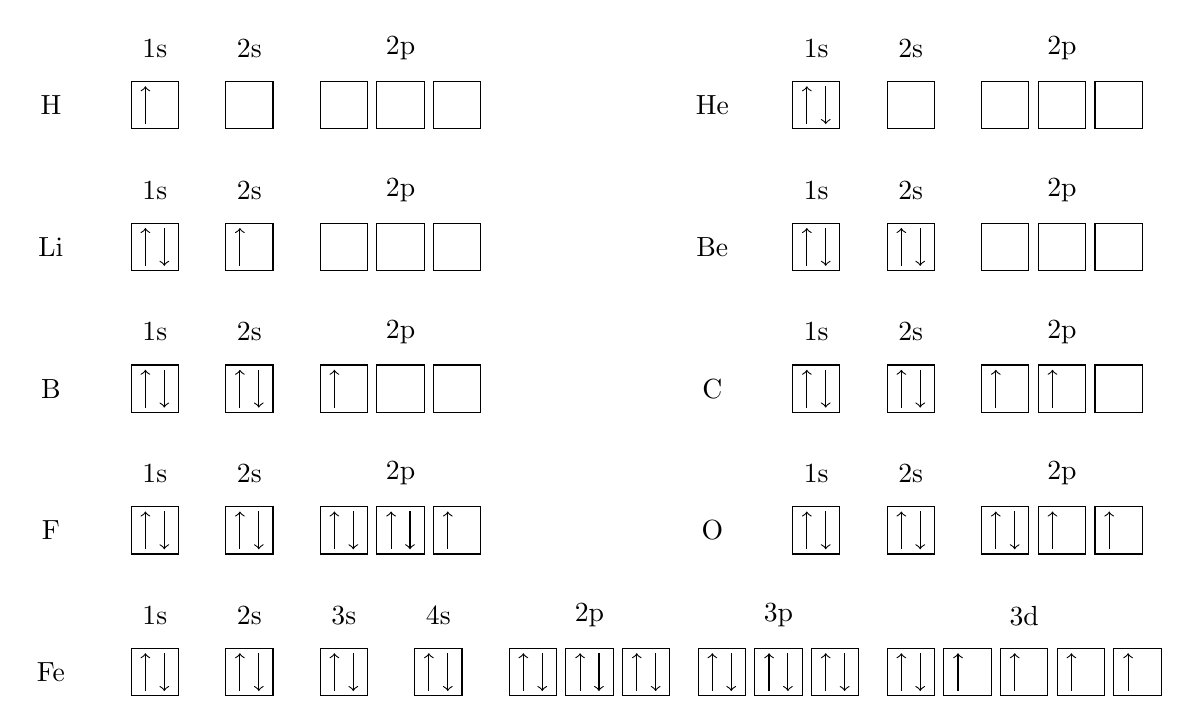
\begin{tikzpicture}[scale=1.2]
    \begin{scope}[shift={(0,-1.5)}]
        \node at (-1,0) {$\mathrm{F}$};

        \node at (0.1,0.6) {1s};
        \node at (1.1,0.6) {2s};
        \node at (2.7,0.6) {2p};
        
        \draw[->] (0,-0.2) -- (0,0.2);
        \draw[->] (0.2,0.2) -- (0.2,-0.2);
        \draw ( -0.15, -0.25) rectangle (0.35,0.25);
        
        \draw[->] (1,-0.2) -- (1,0.2);
        \draw[->] (1.2,0.2) -- (1.2,-0.2);
        \draw (0.85,-0.25) rectangle (1.35,0.25);
        
        \draw[->] (2,-0.2) -- (2,0.2);
        \draw[->] (2.2,0.2) -- (2.2,-0.2);
        \draw (1.85,-0.25) rectangle (2.35,0.25);
        
        \draw[->] (2.6,-0.2) -- (2.6,0.2);
        \draw[->] (2.8,0.2) -- (2.8,-0.2);
        \draw (2.45,-0.25) rectangle (2.95,0.25);
        
        \draw[->] (3.2,-0.2) -- (3.2,0.2);
        \draw (3.05,-0.25) rectangle (3.55,0.25);
    \end{scope}

    \begin{scope}[shift={(7,-1.5)}]
        \node at (-1,0) {$\mathrm{O}$};

        \node at (0.1,0.6) {1s};
        \node at (1.1,0.6) {2s};
        \node at (2.7,0.6) {2p};
        
        \draw[->] (0,-0.2) -- (0,0.2);
        \draw[->] (0.2,0.2) -- (0.2,-0.2);
        \draw ( -0.15, -0.25) rectangle (0.35,0.25);
        
        \draw[->] (1,-0.2) -- (1,0.2);
        \draw[->] (1.2,0.2) -- (1.2,-0.2);
        \draw (0.85,-0.25) rectangle (1.35,0.25);
        
        \draw[->] (2,-0.2) -- (2,0.2);
        \draw[->] (2.2,0.2) -- (2.2,-0.2);
        \draw (1.85,-0.25) rectangle (2.35,0.25);
        
        \draw[->] (2.6,-0.2) -- (2.6,0.2);
        \draw (2.45,-0.25) rectangle (2.95,0.25);
        
        \draw[->] (3.2,-0.2) -- (3.2,0.2);
        \draw (3.05,-0.25) rectangle (3.55,0.25);
    \end{scope}

    \begin{scope}[shift={(0,0)}]
        \node at (-1,0) {$\mathrm{B}$};

        \node at (0.1,0.6) {1s};
        \node at (1.1,0.6) {2s};
        \node at (2.7,0.6) {2p};
        
        \draw[->] (0,-0.2) -- (0,0.2);
        \draw[->] (0.2,0.2) -- (0.2,-0.2);
        \draw ( -0.15, -0.25) rectangle (0.35,0.25);
        
        \draw[->] (1,-0.2) -- (1,0.2);
        \draw[->] (1.2,0.2) -- (1.2,-0.2);
        \draw (0.85,-0.25) rectangle (1.35,0.25);
        
        \draw[->] (2,-0.2) -- (2,0.2);
        \draw (1.85,-0.25) rectangle (2.35,0.25);
        
        \draw (2.45,-0.25) rectangle (2.95,0.25);
        
        \draw (3.05,-0.25) rectangle (3.55,0.25);
    \end{scope}

    \begin{scope}[shift={(7,0)}]
        \node at (-1,0) {$\mathrm{C}$};

        \node at (0.1,0.6) {1s};
        \node at (1.1,0.6) {2s};
        \node at (2.7,0.6) {2p};
        
        \draw[->] (0,-0.2) -- (0,0.2);
        \draw[->] (0.2,0.2) -- (0.2,-0.2);
        \draw ( -0.15, -0.25) rectangle (0.35,0.25);
        
        \draw[->] (1,-0.2) -- (1,0.2);
        \draw[->] (1.2,0.2) -- (1.2,-0.2);
        \draw (0.85,-0.25) rectangle (1.35,0.25);
        
        \draw[->] (2,-0.2) -- (2,0.2);
        \draw (1.85,-0.25) rectangle (2.35,0.25);
        
        \draw[->] (2.6,-0.2) -- (2.6,0.2);
        \draw (2.45,-0.25) rectangle (2.95,0.25);

        \draw (3.05,-0.25) rectangle (3.55,0.25);
    \end{scope}

    \begin{scope}[shift={(0,3)}]
        \node at (-1,0) {$\mathrm{H}$};

        \node at (0.1,0.6) {1s};
        \node at (1.1,0.6) {2s};
        \node at (2.7,0.6) {2p};
        
        \draw[->] (0,-0.2) -- (0,0.2);
        \draw ( -0.15, -0.25) rectangle (0.35,0.25);
        
        \draw (0.85,-0.25) rectangle (1.35,0.25);
        
        \draw (1.85,-0.25) rectangle (2.35,0.25);
        
        \draw (2.45,-0.25) rectangle (2.95,0.25);
        
        \draw (3.05,-0.25) rectangle (3.55,0.25);
    \end{scope}

    \begin{scope}[shift={(7,3)}]
        \node at (-1,0) {$\mathrm{He}$};

        \node at (0.1,0.6) {1s};
        \node at (1.1,0.6) {2s};
        \node at (2.7,0.6) {2p};
        
        \draw[->] (0,-0.2) -- (0,0.2);
        \draw[->] (0.2,0.2) -- (0.2,-0.2);
        \draw ( -0.15, -0.25) rectangle (0.35,0.25);
        
        \draw (0.85,-0.25) rectangle (1.35,0.25);
        
        \draw (1.85,-0.25) rectangle (2.35,0.25);
        
        \draw (2.45,-0.25) rectangle (2.95,0.25);
        
        \draw (3.05,-0.25) rectangle (3.55,0.25);
    \end{scope}

    \begin{scope}[shift={(0,1.5)}]
        \node at (-1,0) {$\mathrm{Li}$};

        \node at (0.1,0.6) {1s};
        \node at (1.1,0.6) {2s};
        \node at (2.7,0.6) {2p};
        
        \draw[->] (0,-0.2) -- (0,0.2);
        \draw[->] (0.2,0.2) -- (0.2,-0.2);
        \draw ( -0.15, -0.25) rectangle (0.35,0.25);
        
        \draw[->] (1,-0.2) -- (1,0.2);
        \draw (0.85,-0.25) rectangle (1.35,0.25);
        
        \draw (1.85,-0.25) rectangle (2.35,0.25);
        
        \draw (2.45,-0.25) rectangle (2.95,0.25);
        
        \draw (3.05,-0.25) rectangle (3.55,0.25);
    \end{scope}

    \begin{scope}[shift={(7,1.5)}]
        \node at (-1,0) {$\mathrm{Be}$};

        \node at (0.1,0.6) {1s};
        \node at (1.1,0.6) {2s};
        \node at (2.7,0.6) {2p};
        
        \draw[->] (0,-0.2) -- (0,0.2);
        \draw[->] (0.2,0.2) -- (0.2,-0.2);
        \draw ( -0.15, -0.25) rectangle (0.35,0.25);
        
        \draw[->] (1,-0.2) -- (1,0.2);
        \draw[->] (1.2,0.2) -- (1.2,-0.2);
        \draw (0.85,-0.25) rectangle (1.35,0.25);
        
        \draw (1.85,-0.25) rectangle (2.35,0.25);
        
        \draw (2.45,-0.25) rectangle (2.95,0.25);
        
        \draw (3.05,-0.25) rectangle (3.55,0.25);
    \end{scope}

    \begin{scope}[shift={(0,-3)}]
        \node at (-1,0) {$\mathrm{Fe}$};

        \node at (0.1,0.6) {1s};
        
        \draw[->] (0,-0.2) -- (0,0.2);
        \draw[->] (0.2,0.2) -- (0.2,-0.2);
        \draw ( -0.15, -0.25) rectangle (0.35,0.25);
        
        \node at (1.1,0.6) {2s};
        \draw[->] (1,-0.2) -- (1,0.2);
        \draw[->] (1.2,0.2) -- (1.2,-0.2);
        \draw (0.85,-0.25) rectangle (1.35,0.25);
        
        \node at (2.1,0.6) {3s};
        \draw[->] (2,-0.2) -- (2,0.2);
        \draw[->] (2.2,0.2) -- (2.2,-0.2);
        \draw (1.85,-0.25) rectangle (2.35,0.25);
        
        \node at (3.1,0.6) {4s};
        \draw[->] (3,-0.2) -- (3,0.2);
        \draw[->] (3.2,0.2) -- (3.2,-0.2);
        \draw (2.85,-0.25) rectangle (3.35,0.25);
        
        \node at (4.7,0.6) {2p};

        \draw[->] (4,-0.2) -- (4,0.2);
        \draw[->] (4.2,0.2) -- (4.2,-0.2);
        \draw (3.85,-0.25) rectangle (4.35,0.25);
        
        \draw[->] (4.6,-0.2) -- (4.6,0.2);
        \draw[->] (4.8,0.2) -- (4.8,-0.2);
        \draw (4.45,-0.25) rectangle (4.95,0.25);
        
        \draw[->] (5.2,-0.2) -- (5.2,0.2);
        \draw[->] (5.4,0.2) -- (5.4,-0.2);
        \draw (5.05,-0.25) rectangle (5.55,0.25);
        
        \node at (6.7,0.6) {3p};

        \draw[->] (6,-0.2) -- (6,0.2);
        \draw[->] (6.2,0.2) -- (6.2,-0.2);
        \draw (5.85,-0.25) rectangle (6.35,0.25);
        
        \draw[->] (6.6,-0.2) -- (6.6,0.2);
        \draw[->] (6.8,0.2) -- (6.8,-0.2);
        \draw (6.45,-0.25) rectangle (6.95,0.25);
        
        \draw[->] (7.2,-0.2) -- (7.2,0.2);
        \draw[->] (7.4,0.2) -- (7.4,-0.2);
        \draw (7.05,-0.25) rectangle (7.55,0.25);
        
        \node at (9.3,0.6) {3d};

        \draw[->] (8,-0.2) -- (8,0.2);
        \draw[->] (8.2,0.2) -- (8.2,-0.2);
        \draw (7.85,-0.25) rectangle (8.35,0.25);
        
        \draw[->] (8.6,-0.2) -- (8.6,0.2);
        \draw (8.45,-0.25) rectangle (8.95,0.25);
        
        \draw[->] (9.2,-0.2) -- (9.2,0.2);
        \draw (9.05,-0.25) rectangle (9.55,0.25);
        
        \draw[->] (9.8,-0.2) -- (9.8,0.2);
        \draw (9.65,-0.25) rectangle (10.15,0.25);
        
        \draw[->] (10.4,-0.2) -- (10.4,0.2);
        \draw (10.25,-0.25) rectangle (10.75,0.25);
    \end{scope}

\end{tikzpicture}
\end{center}

Здесь у гелия 2 электрона на первой s-орбитали, поэтому электронная конфигурация записывается как $1\text{s}^2$. Для железа электронная конфигурация записывается как $1\text{s}^2\ 2\text{s}^2\ 2\text{p}^6\ 3\text{s}^2\ 3\text{p}^6\ 4\text{s}^2\ 3\text{d}^6$

\mediumvspace

Полный момент электрона складывается из орбитального момента $\vec L$ и спинового момента $\vec S$, и называется полным моментом $\vec J = \vec L + \vec S$. Его величина равна

\[
J = \sqrt{j(j+1)} \hbar, \quad j = |l-s|, \dots, l+s.
\]

Когда внутренняя оболочка не заполнена, а заполняется внешняя, электроны имеют несбалансированные спины и орбитальные моменты. Это приводит к образованию так называемых магнитных моментов, из которых складываются макроскопические магнитные свойства вещества. Именно такие элементы, как железо, кобальт и никель, становятся сильными магнитами

\smallvspace

Число квантово-доступных состояний на одном энергетическом уровне определяется формулой $2 n^2$, где $n$ — главное квантовое число. Это учитывает все возможные значения $l$, $m$ и спин $s = \frac12$ для электрона

\smallvspace

Энергетические уровни в атоме могут расщепляться из-за взаимодействий спина и орбитального момента (спин-орбитальное взаимодействие) или из-за внешнего магнитного поля, как в опыте Зеемана. Зееман помещал пламя, в котором были распылены натриевые соли, между полюсами очень сильного магнита. Затем он наблюдал спектр излучения через спектроскоп. Ожидалось, что спектр не изменится -- ведь классическая физика тогда не предсказывала влияния магнетизма на частоты света

Но Зееман заметил, что спектральные линии начали расширяться, а при усилении поля линия раздробилась на несколько компонент. Это стало первым прямым доказательством того, что атомы имеют магнитный момент, а энергетические уровни расщепляются в магнитном поле

\smallvspace

Некоторые переходы между энергетическими уровнями запрещены законом квантовой механики. Например:
\begin{itemize}
    \item Переходы, не удовлетворяющие правилу отбора $\Delta l = \pm 1$ (для орбитального квантового числа)
    \item Переходы, не удовлетворяющие изменению проекции магнитного числа $\Delta m = 0, \pm 1$
    \item Переходы, при которых спин электрона меняется (спин-неразрешённые переходы)
\end{itemize}

Такие запреты определяют спектральные линии атомов, их интенсивность и возможность использования в лазерах, спектроскопии и квантовой электронике

% end physics3_2025_11_10.tex

% begin physics3_2025_11_17.tex





\section{8. Квантовые вычисления}

Идея использовать квантовые элементарные ячейки вместо классических была впервые чётко сформулирована в начале 1980-х годов физиками Фейнманом и Манином. Основная мотивация состояла в том, что классические компьютеры плохо справляются с моделированием квантовых систем, поскольку размерность пространства состояний растёт экспоненциально. Квантовые вычисления, напротив, естественным образом используют суперпозицию и интерференцию состояний, что потенциально обеспечивает высокий параллелизм вычислений.

Квантовая элементарная ячейка называется квантовым битом, или кубитом. Его состояние описывается волновой функцией $\psi$, которая представляется вектором. Базисными состояниями кубита являются $|0\rangle = \begin{pmatrix}1 \\ 0\end{pmatrix}$ или $|1\rangle = \begin{pmatrix}0 \\ 1\end{pmatrix}$


Физическая реализация кубита может быть различной. Например, электрон имеет 3 характеристики: масса, заряд и спин. Спин можно использовать как значение кубита

В классических компьютерах используется двоичная логика, основанная на наличии или отсутствии электрического тока. Такое кодирование обеспечивает высокую помехоустойчивость: небольшие флуктуации напряжения не приводят к ошибке логического состояния. В квантовых системах ситуация иная: состояния чрезвычайно чувствительны к внешним воздействиям, что является одной из ключевых инженерных проблем квантовых вычислений

\meduimvspace

Состояние 0 обозначаются $|0\rangle$, а состояние 1 -- $|1\rangle$

Квантовые ячейки также могут обладать смешанными состояниями $\alpha |0\rangle + \beta |1\rangle$. Такие кубиты могут иметь состояние $|0\rangle$ с вероятностью $|\alpha|^2$, а состояние $|1\rangle$ с вероятностью $|\beta|^2$. Из-за этого $|\alpha|^2 + |\beta|^2 = 1$

Элементы в матричной записи обозначают $\alpha$ и $\beta$. В общем случае $\alpha$ и $\beta$ -- комплексные числа

Для отображения вектора состояния нужно четырехмерное пространство. Так как $|\alpha|^2 + |\beta|^2 = 1$, все физически различимые состояния одного кубита можно представить точками на единичной сфере, так называемой сфере Блоха. При стандартной параметризации $\alpha = \cos\frac{\theta}{2}$ и $\beta = e^{i\varphi}\sin\frac{\theta}{2}$ каждому состоянию соответствует точка с углами $(\theta, \varphi)$

\meduimvspace

Сфера Блоха позволяет визуализировать только один кубит. Так выглядят $|0\rangle$ и $|1\rangle$:

\begin{center}
    \includegraphics[height=8.5cm]{physics3/images/physics3_0_1_states}
\end{center}

\meduimvspace

Квантовый компьютер должен иметь более 1000 хорошо различаемых кубитов и обеспечить условия для приведения входного регистра в исходное основное базисное состояние 

Практический квантовый компьютер должен содержать большое число хорошо различимых кубитов (порядка сотен или тысяч), обеспечивать их инициализацию в заданное базисное состояние и позволять выполнять управляемые операции над ними. Ключевым параметром является когерентность кубитов — время, в течение которого сохраняется квантовая суперпозиция. Типичные времена когерентности составляют миллисекунды или меньше, однако при тактовых частотах порядка гигагерц за это время удаётся выполнить миллионы квантовых операций. Результат вычислений при этом носит вероятностный характер и извлекается посредством измерений

Хотя квантовый регистр физически может быть очень малым по размеру, управление им требует чрезвычайно сложной экспериментальной инфраструктуры: сверхнизких температур, вакуума, экранирования от внешних полей и высокоточной электроники

Квантовые компьютеры находят применение в моделировании молекул и материалов, оптимизационных задачах, машинном обучении и, в частности, в криптографии. Например, алгоритм Шора позволяет эффективно факторизовать большие числа, что делает уязвимыми классические криптографические схемы. В то же время реализация масштабируемых квантовых компьютеров сталкивается с серьёзными технологическими трудностями, и на текущий момент такие устройства находятся на экспериментальной стадии

\meduimvspace

Состояние двух кубитов можно записать так: $(\alpha_0 |0\rangle + \beta_0 |1\rangle) \xor (\alpha_1 |0\rangle + \beta_1 |1\rangle) = \alpha_0 \alpha_1 |00\rangle + \alpha_0 \beta_1 |01\rangle + \beta_0 \alpha_1 |10\rangle + \beta_0 \beta_1 |11\rangle$

Некоторые двухкубитные состояния не допускают представления в виде произведения состояний отдельных кубитов -- такие состояния называются запутанными


Для работы с кубитами также существуют логические операции -- квантовые вентили или гейты. Так как состояние можно представить волновой функцией, то вентиль можно представить оператором (а значит и матрицей)

Однокубитные вентили описываются матрицей $2 \times 2$, двухкубитные -- $4 \times 4$, $n$-кубитные -- $2^n \times 2^n$. Из-за этого матрицы вентилей для больших чисел кубитом занимает очень много памяти

Чтобы получить информацию о состоянии квантовой системы необходимо выполнить его измерение. Для проведения измерений мы должны активно воздействовать на квантовую систему. В результате сразу же после измерения состояние квантовой системы разрушается, 
то есть система переходит в состояние, соответствующее измеренному значению

\meduimvspace

Рассмотрим простейшие квантовые гейты:

\begin{itemize}
    \item Гейт Адамара (Hadamard) -- гейт, который состояние $|0\rangle$ переводит в состояние $\frac{1}{\sqrt{2}} |0\rangle + \frac{1}{\sqrt{2}} |1\rangle$ (то есть с равновероятными состояниями) и описывается матрицей $\frac{1}{\sqrt{2}} \begin{pmatrix}1 & 1 \\ 1 & -1\end{pmatrix}$

    Физически гейт Адамара может быть реализован, например, с помощью переменного магнитного поля, управляющего спином электрона, или короткого лазерного импульса, воздействующего на атом

    На схемах он изображается так:

    \begin{center}
        \begin{quantikz}
            \lstick{$|0\rangle$} & & \gate{H} & & \rstick{$\longrightarrow \frac{1}{\sqrt{2}}(|0\rangle + |1\rangle)$}
        \end{quantikz}
    \end{center}

    Здесь одна строка -- это кубит и примененные к нему гейты. Использование гейта Адамара в литературе называют \enquote{приготовлением кубита}, поскольку он переводит кубит из определённого базисного состояния в квантовую суперпозицию

    Также гейт Адамара переводит состояние $|1\rangle$ в $\frac{1}{\sqrt{2}} |0\rangle - \frac{1}{\sqrt{2}} |1\rangle$

    \begin{center}
        \includegraphics[height=8.5cm]{physics3/images/physics3_hadamard_states}
    \end{center}

    \item Гейт X (или гейт NOT) инвертирует состояние, то есть переводит из $|0\rangle$ в $|1\rangle$ и из $|1\rangle$ в $|0\rangle$. По сути гейт переворачивает состояния на сфере Блоха по оси $OX$, а его матрица равна $\begin{pmatrix}0 & 1 \\ 1 & 0\end{pmatrix}$

    Гейт X изображается так:

    \begin{center}
    \begin{quantikz}
        \lstick{$|0\rangle$} & \gate{X} & & \rstick{$\longrightarrow |1\rangle$} \\
        \lstick{$a|0\rangle + b|1\rangle$} & \gate{X} & & \rstick{$\longrightarrow b|0\rangle + a|1\rangle$}
    \end{quantikz}
    \end{center}

\end{itemize}





% end physics3_2025_11_17.tex

% begin physics3_2025_11_24.tex





\begin{itemize}
    \item Гейт Z меняет знак у состояния $|1\rangle$, его матрица равна $\begin{pmatrix}1 & 0 \\ 0 & -1\end{pmatrix}$

    Гейт Z изображается так:

    \begin{center}
    \begin{quantikz}
        \lstick{$|0\rangle$} & \gate{Z} & & \rstick{$\longrightarrow |0\rangle$} \\
        \lstick{$a|0\rangle + b|1\rangle$} & \gate{Z} & & \rstick{$\longrightarrow a|0\rangle - b|1\rangle$}
    \end{quantikz}
    \end{center}
    
    Гейт $Z$ не меняет вероятности измерения, а изменяет только относительную фазу компонент состояния

    Из этого последовательное применение гейтов H, Z и H эквивалентно X, а H, X и H -- Z

    \begin{center}
    \begin{quantikz}
        \lstick{$a|0\rangle + b|1\rangle$} & \gate{H} & \gate{Z} & \gate{H} & \rstick{$\longrightarrow a|0\rangle + b|1\rangle$}
    \end{quantikz}
    \end{center}

    \item Гейт Y вращает состояние вокруг оси $OY$ и имеет матрицу $\begin{pmatrix}0 & -i \\ i & 0\end{pmatrix}$

    \begin{center}
    \begin{quantikz}
        \lstick{$a|0\rangle + b|1\rangle$} & \gate{Y} & & \rstick{$\longrightarrow -i b|0\rangle + i a|1\rangle$}
    \end{quantikz}
    \end{center}

    Из этого применения гейтов H, Y и H эквивалентно -Y

    \item Гейт CNOT (от Controlled NOT) применяется на два кубита: один из них управляющий, другой -- управляемый. Если управляющий кубит равен единице, то управляемый бит инвертируется, как после применения гейта X:

    \begin{center}
    \begin{quantikz}
        \lstick{$a|0\rangle + b|1\rangle$} & \ctrl{1} & & \rstick[2]{$ac |00\rangle + ad |01\rangle + bd |10\rangle + bc |11\rangle$} \\
        \lstick{$c|0\rangle + d|1\rangle$} & \gate{X} & & 
    \end{quantikz}
    \end{center}

    Гейт CNOT имеет матрицу $\begin{pmatrix}1 & 0 & 0 & 0 \\ 0 & 1 & 0 & 0 \\ 0 & 0 & 0 & 1 \\ 0 & 0 & 1 & 0\end{pmatrix}$

    Если управляющий бит имеет состояние $\frac{1}{\sqrt{2}} |0\rangle + \frac{1}{\sqrt{2}} |1\rangle$, то управляемый кубит инвертирует значение с вероятностью 50\%

    С помощью этого гейта кубиты можно запутать -- измерение одного из них переводит другой в определенное состояние:

    \begin{center}
    \begin{quantikz}
        \lstick{$a|0\rangle + b|1\rangle$} & \ctrl{1} & & \rstick[2]{$a |00\rangle + b |11\rangle$} \\
        \lstick{$|0\rangle$} & \gate{X} & & 
    \end{quantikz}
    \end{center}

    Аналогично запутывать можно и большее число кубитов
\end{itemize}

Из-за свойства гейта CNOT можно увести кубиты на огромное расстояние, и, измерив один кубит, мы можем узнать значение другого

Из этого можно сделать миллион пар таких кубитов, которые будут передавать информацию. Передачу квантового состояния на расстояние запутанной пары кубитов называют квантовая телепортацией

Допустим Алиса хочет передать кубит с состоянием $|psi\rangle = \alpha |0\rangle + \beta |1\rangle$ Бобу. У Боба есть приемник -- третий кубит, а второй кубит является вспомогательным у Алисы и связан с третьим

Боб с третьим кубитом уезжает на другую планету. 

Получаем трехкубитовую систему: $\frac{1}{\sqrt{2}} (\alpha|000\rangle + \alpha|011\rangle + \beta|011\rangle + \beta |111\rangle)$

После применения еще нескольких гейтов, мы получаем такое состояние: 

\[\frac{1}{2} \left(|00\rangle (\alpha |0\rangle + \beta |1\rangle) + |01\rangle (\alpha |1\rangle + \beta |0\rangle) + |10\rangle (\alpha |0\rangle - \beta |1\rangle) + |11\rangle (\alpha |1\rangle - \beta |0\rangle)\right)\]

Как видно, только в одном случае из четырех третий кубит имеет такое же состояние, что и первый. В остальных случаях Бобу нужно применить соответствующее преобразование (гейтами Z или X), чтобы получить значение с точностью до знака

Если Алиса измерила свои кубиты и получила $00$, то информация доставлена успешна

\begin{center}
\begin{quantikz}
    \lstick{$|\psi\rangle$} & & & \ctrl{1} & \gate{H} & & \ctrl{2} & & \rstick[2]{$\text{Кубиты Алисы}$}\\
    \lstick{$|0\rangle$} & \gate{H} & \ctrl{1} & \gate{X} & & \ctrl{1} & & & \\
    \lstick{$|0\rangle$} & & \gate{X} & & & \gate{X} & \gate{Z} & \meter{} & \rstick{$\text{Кубит Боба}$}
\end{quantikz}
\end{center}

Проблема в том, что третий гейт CNOT должен быть реализован на этом огромном расстоянии. Запутанность не позволяет передавать информацию мгновенно. Хотя измерение одного кубита мгновенно определяет состояние другого, результат измерения является случайным и не может быть использован для передачи сигнала

Помимо этого, неизвестное квантовое состояние невозможно скопировать на другой кубит. Это утверждение известно как теорема о запрете клонирования и следует из линейности квантовой механики


% end physics3_2025_11_24.tex

% begin physics3_2025_12_01.tex





\section{9. Квантово-механическое описание молекул и статистика частиц}

Из курса школьной химии известно, что есть два вида связи между атомами в молекуле:

\begin{itemize}
    \item Ионная (или гетерополярная) -- осуществляется кулоновским электростатическим взаимодействием ионов противоположных знаков, например $\mathrm{Na}\mathrm{Cl} \ (\mathrm{Na}^+\mathrm{Cl}^-)$ или $\mathrm{K}\mathrm{Br} \ (\mathrm{K}^+\mathrm{Br}^-)$. Электрон в этом случае в среднем локализован около одного из атомов, а связь имеет в основном электростатическую природу
    \item Ковалентная (или гомеополярная) -- образуется парами электронов с противоположными спинами в таких молекулах, как $\mathrm{O}_2$, $\mathrm{N}_2$, $\mathrm{CN}$, электроны значительную часть времени проводят в пространстве между атомами и являются \enquote{общими} для обоих ядер
\end{itemize}

Рассмотрим подробнее, как возникает ковалентная связь на примере молекулы водорода. При сближении атомов водорода наступает перекрывание электронных областей и возникает новое состояние, которое не свойственно системе изолированных атомов

Однако на самом деле происходит перераспределение плотности вероятности, и вероятность того, что электрон находится между ядрами, близка к единице. Именно это приводит к уменьшению энергии системы: электроны экранируют кулоновское отталкивание протонов и одновременно притягиваются к обоим ядрам

Здесь принцип Паули утверждает, что в одной области не может быть электронов с теми же квантовыми числами, то есть эти два электрона, находящиеся на одном уровне, должны отличаться спином

Если спины электронов противоположны, полная волновая функция системы оказывается симметричной по пространственным координатам, и плотность вероятности между ядрами велика -- связь образуется. Если же спины электронов одинаковы, пространственная часть волновой функции становится антисимметричной. В этом случае волновая функция обращается в нуль в области между ядрами, вероятность нахождения там электронов резко уменьшается, и энергетически выгодной связи не возникает

Составим уравнение Шрёдингера для ковалентной связи в молекуле $\mathrm{H}_2$

% https://www.geogebra.org/calculator/hkcemf2v

\begin{center}
    \includegraphics[width=10cm]{physics3/images/physics3_h2_model}
\end{center}


Тут $e_1$ и $e_2$ -- электроны, а $A$ и $B$ -- протоны. Функция потенциала будет выглядеть так: $U = \frac{e^2}{4\pi \varepsilon_0} \left(\frac{1}{R} + \frac{1}{r_{12}} - \frac{1}{r_{1a}} - \frac{1}{r_{1b}} - \frac{1}{r_{2a}} - \frac{1}{r_{2b}}\right)$. Здесь $r_{12}$ -- расстояние между электронами, $R$ -- расстояние между протонами, а $r_{1a}$ -- расстояние между электроном и ядром

А уравнение Шрёдингера будет выглядеть так: $\Delta_1 \Psi + \Delta_2 \Psi + \frac{2m}{\hbar^2} (E - U) \Psi = 0$

Здесь волновая функция $\Psi$ зависит от координат обоих электронов. Собственные значения энергии зависят от расстояния между ядрами $R$:

% https://www.geogebra.org/calculator/kj3rqpr8

\begin{center}
    \includegraphics[width=12cm]{physics3/images/physics3_energy_functions_h2}
\end{center}

График $E(R)$ имеет минимум, соответствующий устойчивой молекуле. Глубина этого минимума определяет энергию диссоциации $E_0$ -- энергию, которую необходимо сообщить молекуле, чтобы разорвать связь и получить два свободных атома водорода

3-ье состояние -- это возбужденное состояние, в котором расстояние между ядрами больше, электроны находятся на орбиталях высоких порядков, что позволяет молекуле держатся при большем расстоянии между ядрами

В газе молекулы, помимо электронных состояний, обладают поступательным, вращательным и колебательным движением. Каждому виду движения соответствуют свои квантованные энергетические уровни. Вращательные уровни связаны с квантуемым моментом импульса молекулы, а колебательные — с квантованием движения ядер около положения равновесия. В результате каждому электронному уровню соответствует большое число близко расположенных уровней вращения и колебаний

В адиабатическом приближении волновую функцию молекулы можно представить в виде произведения трёх независимых сомножителей:
$\Psi = \psi_e \cdot \psi_v \cdot \psi_r$

Электронная часть волновой функции $\psi_e$ описывает распределение электронов в поле практически неподвижных ядер. В этой функции межъядерное расстояние $R$ выступает как параметр, а не как динамическая переменная. Решение электронного уравнения Шрёдингера даёт собственные значения энергии $E_e(R)$, которые зависят от $R$ и образуют потенциальную кривую взаимодействия ядер

Колебательная волновая функция $\psi_v(R)$ описывает движение ядер вдоль линии связи, то есть колебания молекулы около равновесного межъядерного расстояния $R_0$, соответствующего минимуму потенциальной кривой $E_e(R)$. Вблизи этого минимума потенциал можно разложить в ряд по $(R - R_0)$ и в первом приближении считать гармоническим. Тогда колебательные уровни энергии имеют вид $E_v = \hbar \omega \left(v + \tfrac{1}{2}\right), v = 0,1,2,\dots$, что соответствует квантовому гармоническому осциллятору

Вращательная волновая функция $\psi_r(\theta,\varphi)$ описывает вращение молекулы как целого вокруг центра масс. Для двухатомной молекулы эта задача эквивалентна вращению жёсткого ротатора, и вращательные уровни энергии определяются выражением $E_r = \frac{\hbar^2}{2I} J(J+1), J = 0,1,2,\dots$, где $I$ — момент инерции молекулы. Собственные функции вращательного движения выражаются через сферические гармоники

Таким образом, полная энергия молекулы в этом приближении представляется суммой электронной, колебательной и вращательной энергий: $E \approx E_e + E_v + E_r$


Переходы между этими уровнями сопровождаются поглощением или испусканием фотонов, что приводит к сложным спектрам поглощения и пропускания, например, переходы электронных энергии дают фотоны с длиной волны в ультрафиолетовом диапазоне и так далее. Анализ таких спектров позволяет определить межъядерные расстояния, моменты инерции молекул, силовые константы связей и массы ядер. Например, спектр пропускания молекулы $^{13}\mathrm{C}^{16}\mathrm{O}_2$ содержит характерные полосы, связанные с колебательно-вращательными переходами

\bigvspace

Описать движение молекул газа с помощью методов классической механики представляет из себя сложной задачей из-за числа уравнений. Поэтому используются статистические методы

В XIX веке физик Максвелл создал теорию того, как распределяется скорость молекул газа:

% https://www.geogebra.org/calculator/mu2u7wbu

\begin{center}
    \includegraphics[width=12cm]{physics3/images/physics3_maxwell_distribution}
\end{center}

Функция плотности распределения выглядит так: $f(v) = A v^2 e^{-\frac{mv^2}{2kT}}$, где $m$ -- масса молекулы, $T$ -- температура, $k$ -- постоянная Больцмана, а $A$ -- коэффициент нормировки

Это распределение показывает, что в газе существует наиболее вероятная скорость, а также медленные и быстрые молекулы

Другой, более общий подход предложил Больцман. Частицы подчиняются разными статистическими закономерностями в зависимости от того, целый ли его спин или полуцелый

Если при перестановке координат двух частиц выполняется $|\Psi(x_1, x_2)|^2 = |\Psi(x_2, x_1)|^2$, то получаем $\Psi(x_1, x_2) = \Psi(x_2, x_1)$ или $\Psi(x_1, x_2) = -\Psi(x_2, x_1)$

То есть волновая функция частиц с целым спином симметрична (то есть первое решение) -- такая статистика называется статистикой Бозе-Эйнштейна, а рассматриваемые частицы -- бозоны. Для бозонов вероятность того, что при добавлении в систему нового бозона он займет $i$-ое состояние, пропорциональна корню из числа заполнения этого состояния $p_i \sim \sqrt{N_i}$

Если частицы имеют полуцелый спин, то она называются фермионами, функция получается антисимметричной, а статистика называется статистикой Ферми-Дирака, функция распределения для нее выглядит так: $n_i(E_i) = \frac{1}{e^{\frac{E_i - \mu}{kT}} + 1}$, где $n_i$ -- среднее число фермионов в системе с энергией $E_i$

Для фермионов справедлив принцип Паули: если две частицы находятся в одинаковом состоянии, то их волновая функция не может менять знак при их перестановке. Из-за этого $0 \leq n_i \leq 1$

% https://www.geogebra.org/calculator/afv5jygp

\begin{center}
    \includegraphics[width=12cm]{physics3/images/physics3_fermi_stats}
\end{center}

Важной величиной в статистической физике является химический потенциал $\mu = \frac{dE}{dN}$, который показывает, на сколько изменяется энергия системы при добавлении одной частицы. Для ферми-газа при температуре $T \to 0$ все состояния с энергией $E < \mu$ заняты ($n_i(E) \to 1$), а состояния с $E > \mu$ свободны ($n_i(E) \to 0$)

При $T = 0$ статистика имеет такой вид:

% https://www.geogebra.org/calculator/afv5jygp

\begin{center}
    \includegraphics[width=12cm]{physics3/images/physics3_fermi_stats_t_0}
\end{center}

Здесь значения разлома функции называется энергией Ферми. До нее состояния считаются занятыми (то есть вероятность найти фермион с $E < E_F$ высока), а после нее свободными (то есть новый фермион свободно может занять его)

Энергия Ферми равна $E_F = \frac{\hbar^2}{8m} \left(\frac{3n}{\pi}\right)^{\frac{2}{3}}$

Если разделить $E_F$ на постоянную Больцмана $k$, получим $T_F = \frac{E_F}{k}$ -- температура Ферми. Для металлов, например, температура Ферми примерно равна $T_F = 10^6 \text{К}$

При повышении температуры резкий переход в распределении Ферми–Дирака сглаживается: электроны вблизи уровня Ферми могут переходить на более высокие энергетические уровни за счёт тепловой энергии

Эти квантово-статистические эффекты лежат в основе работы многих современных устройств, в том числе полупроводниковых приборов и светодиодов

% end physics3_2025_12_01.tex

% begin physics3_exam_list.tex
\clearpage

\section{X. Программа экзамена в 2024/2025}

\begin{enumerate}
    \item Электромагнитная плоская монохроматическая волна волна и ее характеристики: вектора $E$, 
$B$ и $k$, амплитуда, поляризация, фаза, длина волны и фазовая скорость. Длина волны и 
фазовая скорость в вакууме и среде. 
    \item Поляризация. Степень поляризации. Закон Малюса. 
    \item Линейная, круговая и эллиптическая поляризации. Способы получения и преобразования 
одной в другую.  
    \item Сложение двух бегущих, в одном направлении плоских монохроматических волн с близкими 
частотами. Простейший волновой пакет - биения. Фазовая и групповая скорости волн.  
    \item Сложение электромагнитных волн с непрерывным спектром по частотам. Волновой пакет. 
Групповая скорость.  
    \item Волновой пакет. Локализация волнового пакета и его длительность. 
    \item Дисперсия групповой скорости. Расплывание волнового пакета в среде. Оценка времени 
расплывания.  
    \item Фотоэффект. Законы фотоэффекта. Уравнение Эйнштейна. 
    \item Эффект Комптона. 
    \item Корпускулярно волновой дуализм. Волна де-Бройля. Волновая функция и ее физическая 
интерпретация.  
    \item Основные постулаты квантовой механики. Операторы координаты и импульса.  
    \item Коммутационные соотношения координаты - проекции импульса. Соотношения 
неопределенностей.  
    \item Гамильтониан. Оператор полной энергии в координатном представлении.  
    \item Нестационарное и стационарное уравнение Шредингера.  
    \item Прохождение квантовой частицы энергетического барьера. Туннелирование.  
    \item Частицы в потенциальной яме с бесконечными стенками. Энергетические уровни. 
    \item Уравнение Шредингера для частицы в параболическом потенциале. Уровни энергии и 
волновые функции квантового гармонического осциллятора.  
    \item Оператор орбитального момента (момента импульса) в декартовых и сферических 
координатах. Собственные значения $z$-й проекции оператора орбитального движения 
электрона.  
    \item Операторы полного орбитального момента и квадрата орбитального момента. Собственные 
значения операторов. Коммутационные отношения между ними.  
    \item Атом водорода. Построение решения для задачи движения электрона в атоме водорода. 
Разделение волновой функции на радиальную и угловую части.  
    \item Атом водорода без учета спина. Квантовые числа. Уровни энергий. Вырождение энергии по 
орбитальному квантовому числу.  
    \item Опыт Штерна-Герлаха. Гиромагнитное отношение. Магнетон Бора. 
    \item Спин электрона. Оператор спина электрона. Собственный магнитный момент электрона 
    \item Физические системы для квантовой информации (двумерные кубиты). Базисные состояния 
для фотонных и спиновых систем.  
    \item Сфера Блоха и представление кубита на сфере Блоха.  
    \item Запутанные состояния для двух частичных квантовых систем и их отличие состояний двух 
невзаимодействующих систем.  
    \item Статистика Ферми-Дирака. Энергия Ферми. 
    \item Модель Кронига-Пенни. Энергетические зоны. 
    \item Заполнение зон чистого полупроводника. Донорная и акцепторная примесь. Изменения в 
структуре зон. 
    \item pn-переход. Прямое и обратное смещение. Полевой транзистор.
\end{enumerate}

% end physics3_exam_list.tex



\end{document}

